\documentclass[12pt]{article}
\usepackage[margin=0.6in]{geometry}
\usepackage{graphicx}
\usepackage{subcaption}
\usepackage{sidecap}
\usepackage{amsfonts}
\usepackage{amsmath}
\usepackage{amssymb}
\usepackage{psfrag}
\usepackage{float}
\usepackage{algorithm} 
\usepackage{algorithmic}
\usepackage{epstopdf}
\usepackage{hyperref}
\usepackage{soul,color}

\newcommand{\defeq}{\stackrel{\triangle}{=}}

\begin{document}

	\tableofcontents
	
	\section{SAG}
	SAG is originally developed for deterministic optimization problems of the form 
	\begin{equation}
		\label{saa}
 		\hat{F}(\theta) \defeq \frac{1}{m} \sum_{i=1}^{m}  f_i(\theta).
	\end{equation}
	
	The main iteration of the algorithm is given by 

 \begin{align*}
   \mbox{sample } i& \mbox{ from } \{1,\ldots,m\}  \\
   y_i &= \nabla f_i(\theta^k) \\
   \hat{g_k} &= \frac{1}{m} \sum_{i=1}^m y_i , \\ 
   \theta^{k+1} &= \theta^k - \alpha_k \hat{g_k}
 \end{align*}
 
 	This method requires $\{y_1,\ldots,y_m\}$ initialized and stored. Note that the sampling scheme for $i$ can be either with or without replacement. 
 
  \subsection{Initialization 1 : SGD}
  
  A full cycle of SGD is made, to initialize the memory. This CANNOT be represented in the ERG framework.
  
  \subsection{Initialization 2 : Average Gradient (a)}
  
  A full cycle of average gradient descent is done, to initialize the memory. This can be represented in the ERG framework by using $s_k=0$, $u_k=1$.
  
  \subsection{Initialization 3 : Average Gradient (b)}
  
  Sampling with replacement on the full dataset is done, and gradient average is computed based on the number of distinct datapoints sampled. Replacement can occur early on. This CANNOT be represented in the ERG framework, since samples can be drawn from either the sampled or the unsampled sets. This is the way it is done in Mark Schmidt's code. 
  
	\section{ERG}
	
	This modification of the SAG method allows for gradual increase in the memory required, and allows sampling more than one datapoint at each iteration. These two related but different concepts are controlled by two sequences. The sample size from the seen datapoints $\{ s_k\} $, and the sample size from the unseen datapoints $\{ u_k \}$. The requirements are that $s_k \leq \|I_{k-1 }\|$, $u_k \leq \|\{1,\ldots,m\} \setminus I_{k-1}\|$ and $s_k + u_k \leq m$. 
	
	One additional sequence $\{r_k\}$ of indices to remove can be specified. If it is not specified, we set $r_k=0$.
	
	The initialization requires sequences $\{ s_k\} $,$\{ u_k \}$,  $\theta^0$, $\alpha_k$.  $I_0 = \emptyset$.
	At every iteration:
	
 	\begin{align*}
	S_k &=  \mbox{sample of } s_k \mbox{ indices from } I_{k}\\
	\mbox{replace } y_i &= \nabla f_i(\theta^k) \mbox{ for all } i \in S_k \\
	U_k &=  \mbox{sample of } u_k \mbox{ indices from } \{1,\ldots,m\} \setminus I_{k}\\
	\mbox{compute } y_i &= \nabla f_i(\theta^k) \mbox{ for all } i \in U_k \\
	I_{k+1} &=  I_{k} \cup U_k\\
	\hat{g_k} & = \frac{1}{\| I_k \| } \sum_{i \in I_k} y_i \\ 
   	\theta^{k+1} &= \theta^k - \alpha_k \hat{g_k}\\
	R_k &=  \mbox{sample of } r_k \mbox{ indices from } I_{k+1}\\
	I_{k+1}&= I_{k+1} \setminus R_k \\
 	\end{align*}
	
	Two drawbacks are: this method is biased towards the samples included in $I$ early on. In addition, the required memory can approach $m$, and become unmanageable. 
	
	This method is in itself a strategy to fill up the gradient memory from zero.
	
	Some special cases are:
	
	\begin{itemize}
		\item $s_k=0$ and $u_k=1$ with $I_0 = \emptyset$ gives a single pass of averaged gradient method \\
		\item $s_k=1$ and $u_k=0$ with $I_0 = \{1,\ldots,m\}$ gives standard SAG. Note that this requires an existing memory of all $y_i$  \\
	\end{itemize}
 
	\section{ERG - example 1 }
	
	In this simple scheme, we always sample one datapoint from the seen set, and one from the useen set. This corresponds to $s_k = 1$ and $u_k=1$. To keep sequence $s_k$ constant, we require $\|I_0\| = 1$ (and thus, a single gradient is already stored). Every iteration is given by 

 	\begin{align*}
   	\mbox{sample } i& \mbox{ from } I_{k-1}  \\
	\mbox{replace } y_i &= \nabla f_i(\theta^k) \\
	\mbox{sample }  j& \mbox{ from }\{1,\ldots,m\} \setminus I_{k-1}\\
	\mbox{compute }  y_j &= \nabla f_j(\theta^k) \\
	I_k &=  I_{k-1} \cup j\\
	\hat{g_k} & = \frac{1}{\| I_k \| } \sum_{i \in I_k} y_i \\ 
   	\theta^{k+1} &= \theta^k - \alpha_k \hat{g_k}
 	\end{align*}
	
	
	  The only parameter in the example above is the steplength $\alpha_k$. 
 
  	\section{ERG - example 2}
	
  	Here we increase batchsizes by setting $s_k = k$ and $u_k=k$. We require $\|I_0\| = 1$. Every iteration is given by 
	
 	\begin{align*}
	S_k &=  \mbox{sample of } k \mbox{ indices from } I_{k-1}\\
	\mbox{replace } y_i &= \nabla f_i(\theta^k) \mbox{ for all } i \in S_k \\
	U_k &=  \mbox{sample of } k \mbox{ indices from } \{1,\ldots,m\} \setminus I_{k-1}\\
	\mbox{compute } y_i &= \nabla f_i(\theta^k) \mbox{ for all } i \in U_k \\
	I_k &=  I_{k-1} \cup U_k\\
	\hat{g_k} & = \frac{1}{\| I_k \| } \sum_{i \in I_k} y_i \\ 
   	\theta^{k+1} &= \theta^k - \alpha_k \hat{g_k}
 	\end{align*}
	
	
  	  The only parameter in the example above is the steplength $\alpha_k$.
	\section{CSAG}
	
	The objective is to minimize a stochastic function
	\begin{equation}
		\label{prob}
		\min_{\theta} F(\theta) = \mathbb{E}_{x,y}[ f(\theta;x,y)],
	\end{equation}
	where training examples $(x,y)$ are available on demand. Furthermore, assume $y$ (which we call the \emph{class}) is known to take on one of a few values in the finite set $\{c_1,...,c_C\}$. We call the parameter $C$ the \emph{number of classes}.\\
	We build the estimate of the gradient of $F$ by keeping track of the previous gradients for each class, and replace them as new gradient samples are computed. Thus, the memory requirement is linearly dependent on the number of classes, and not on the total number of available datapoints. \\
	The optimization iteration is given by	
	 \begin{align}
	   \mbox{sample } & (x,y) \\
	   \mbox{compute } &g_k \mbox{ as a function of }(x,y,\theta^k) \\
	   h_y &= g_k  \\
	   \hat{g_k} &= \frac{1}{C} \sum_{i \in \{c_1,...,c_C\}} h_i , \\
	   \theta^{k+1} &= \theta^k - \alpha_k \hat{g_k}
	 \end{align}
	For a binary classification problem with only two datapoints available, the gradient estimate becomes exact, while a stochastic gradient method is wild.\\
	Weighting according to a) number of observed examples from each class b) age of the estimates, can be appropriate.
	 
	
	Some special cases are:
	
	\begin{itemize}
		\item $y = \emptyset$. This corresponds to SGD. \\
		\item $x = \emptyset$. This corresponds to SAG. \\
	\end{itemize}
	

	
	\section{Combination of The Two Ideas}
	
	Combining CSAG and ERG is straightforward, since they deal with unrelated properties of the SAG algorithm. We simply update by class rather the individual datapoints. 
	
		
	\section{Use in quasi-newton}
	The strategies described above are methods that approximate gradients at each iteration. These are the only objects needed in a (stochastic) quasi-newton algorithm. The only difficulty arises when hessian-vector products are required as well, but a simple version can be implemented without change. 
		
	\section{Theory}
	
	\newpage 
	
	\section{SAG-like idea: Eliminate Dependence on $m$}
	 The method is appropriate for problem 
	\begin{equation}
		\min_{\theta} F(\theta) = \mathbb{E}_{z}[ f(\theta;z)].
	\end{equation}
	Assume we have memory capacity $M$, i.e. we are able to efficiently store and retreive $M$ gradient estimates. Here we store full vectors, as there is no efficient way to store gradient averages. Using this capability, we define $\hat{g_k}$ to be the average of the previously seen $M_k \leq M$ minibatch gradient estimates. The optimization iteration is given by	
	 \begin{align}
	   \mbox{choose } & s_k \\
	   \mbox{choose } & M_k \\
	   \mbox{sample } &s_k < \infty \mbox{ training points } z \\
	   \mbox{Replace the oldest }  &g_i \mbox{ with the new mini-batch estimate}\\
	   \hat{g_k} &= \frac{1}{M_k} \sum_{i=1}^{M_k} g_i, \\
	   \theta^{k+1} &= \theta^k - \alpha_k \hat{g_k}
	\end{align}
	
	A sample size $s_k$ is needed at each iteration.
	
	
	\section{SAG-like idea: Another Way to  Eliminate Dependence on $m$}
	 The method is appropriate for problem
	\begin{equation}
		\min_{\theta} F(\theta) = \mathbb{E}_{z}[ f(\theta;z)].
	\end{equation}
	Assume we have memory capacity $M$, i.e. we are able to efficiently store and retreive $M$ gradient estimates. Using this capability, we define $\hat{g_k}$ to be the average of the previously seen $M$ stochastic gradients. The optimization iteration is given by	
	 \begin{align}
	   \mbox{sample } &s_k \leq M \mbox{ training points } z \\
	   \mbox{Replace } & s_k \mbox{ of the oldest seen estimates $g_i$ with the new ones}\\
	   \hat{g_k} &= \frac{1}{M} \sum_{i=1}^{M} g_i, \\
	   \theta^{k+1} &= \theta^k - \alpha_k \hat{g_k}
	\end{align}
	The idea of replacing old estimates is present, but without specific requirements on the storage capacity. Every step has costs identical to the original SAG algorithm. The attractive feature of storing structured information about the function is lost, since valuable gradients will be dropped from memory.\\
		
	 
	 
	\section{Idea in Johnson and Zhang}
	Does not require storage of all gradients.
	
	SVRG method.
	
	The optimization iteration is given by	
		 \begin{align}
		   \mbox{sample } & i_t \\
		   w_t &= w_{t-1} - \eta (  \nabla \psi_{i_t} (w_{t-1}) -   \nabla \psi_{i_t} (\tilde{w})  +\tilde{\mu} )
		\end{align}
		
		Where $\tilde{\mu}$ is updated every $m$ iterations by 
		\begin{equation}
			\tilde{\mu} = \frac{1}{n} \sum_{i=1}^{n} \nabla \psi_i(\tilde{w}),
	    \end{equation}
		and $\tilde{w}$ is a fixed $w$ estimate for the next $m$ iterations.
		
		Therefore every outer iteration requires at least a full pass over the data. 
		\newpage
	\section{Numerical Experiments}
	
	\subsection{3 ssag runs}
	This test was conducted on the random logisitic regression problem (Yoram) with L2 regularization parameter $\gamma = 10^{-2}$. 50 variables, 7000 training datapoints, 3000 testing datapoints. Optimal steplengths were chosen, with values of $2^{-7}$, $2^{-8}$, and $2^{-5}$ respectively. I ran it for half an epoch, in order to not run into problems with the second choice of $u_k$. Even linear increase in $s_k$ was too slow.
	\begin{center}
	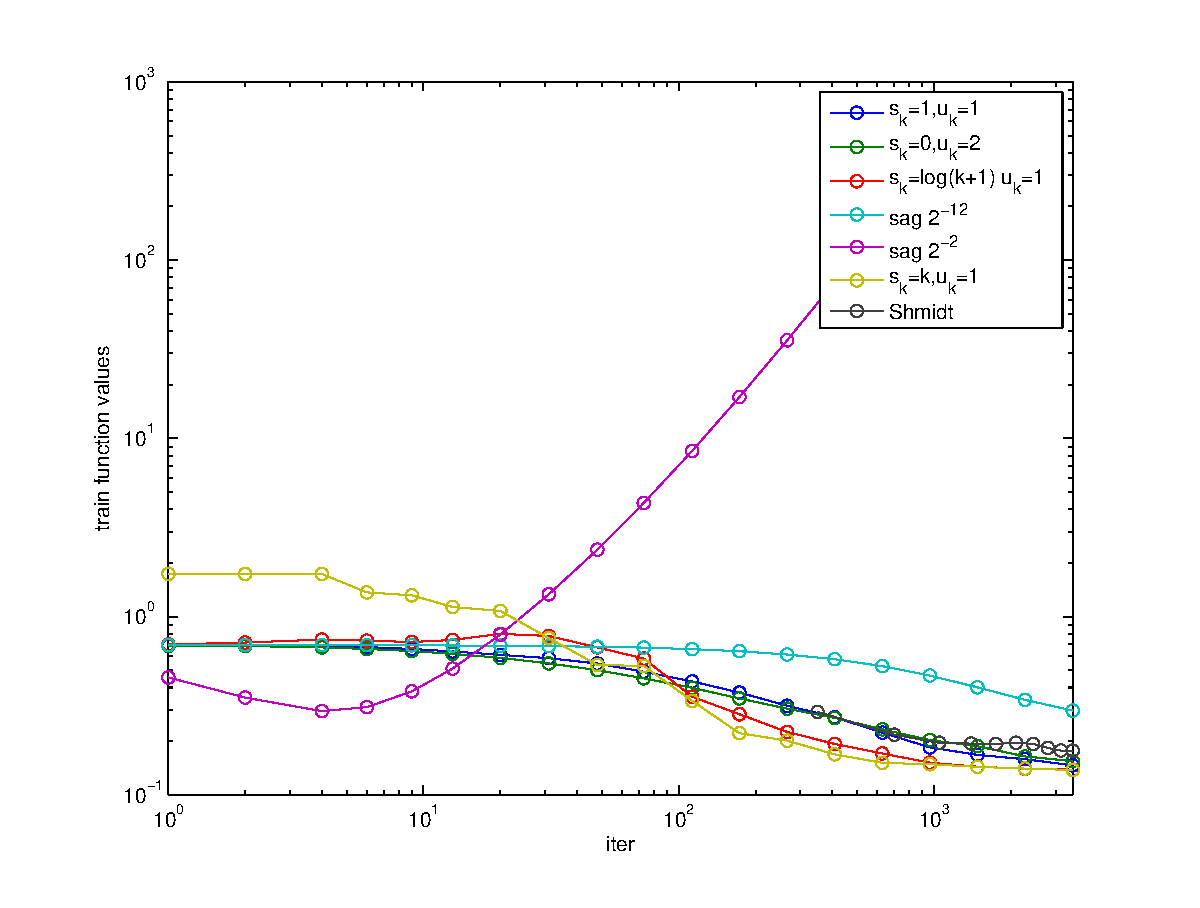
\includegraphics{Figures/12-1-log.eps} 
	\end{center}	
	\begin{center}
	\includegraphics{Figures/12-1-nolog.eps} 
	\end{center}
	\begin{center}
	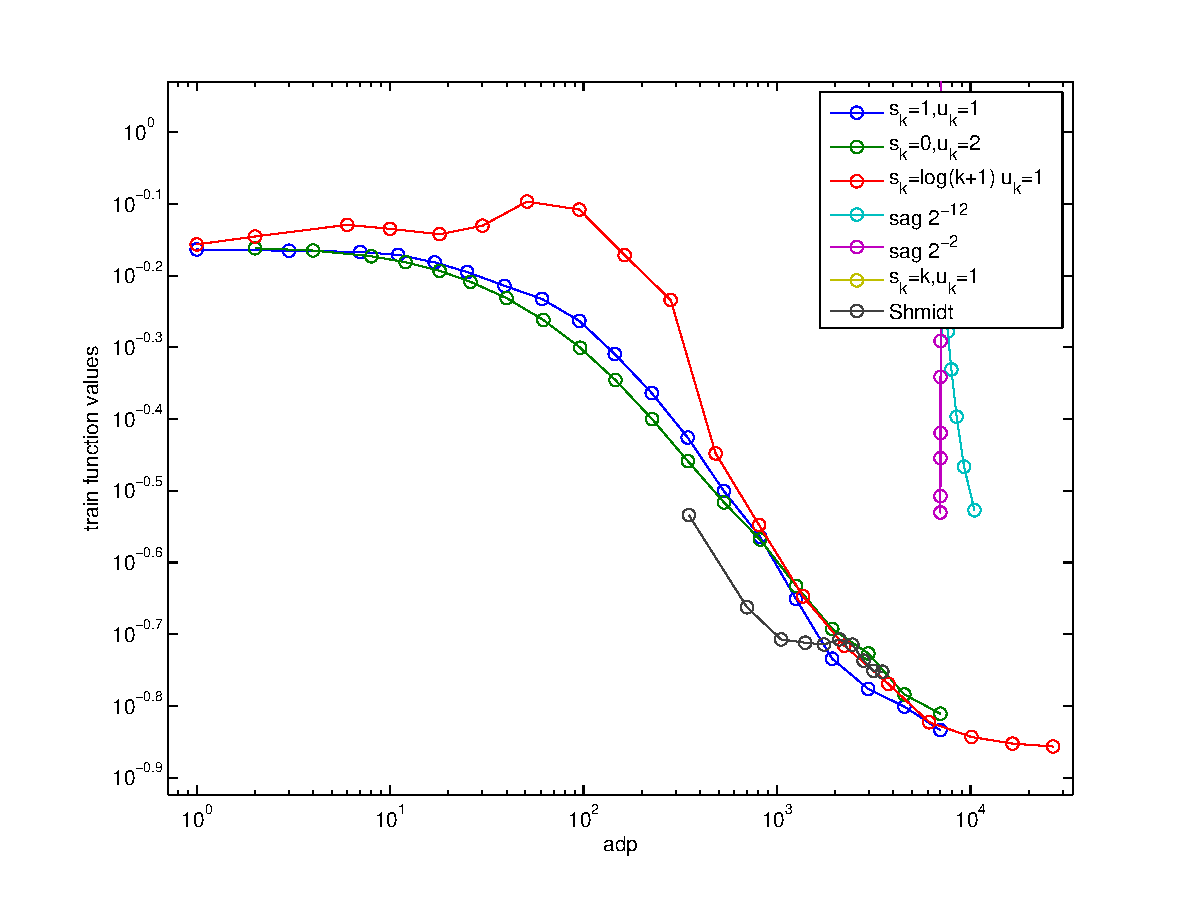
\includegraphics{Figures/adp-log.eps} 
	\end{center}
\subsection{sag in ssag framework}
	Same optimization problem. Varying steplengths are shown for the ssag framework. The method tries to mimic the original sag algorithm, by setting
	\begin{align*}
		u_k = m &\mbox{ if } k=0\\
		u_k = 0 &\mbox{ if } k>0
		\end{align*}
		and $s_k = \min{k,1}$. Number of iterations is $10 m$ where $m$ is the size of the training set. 
	\begin{center}
	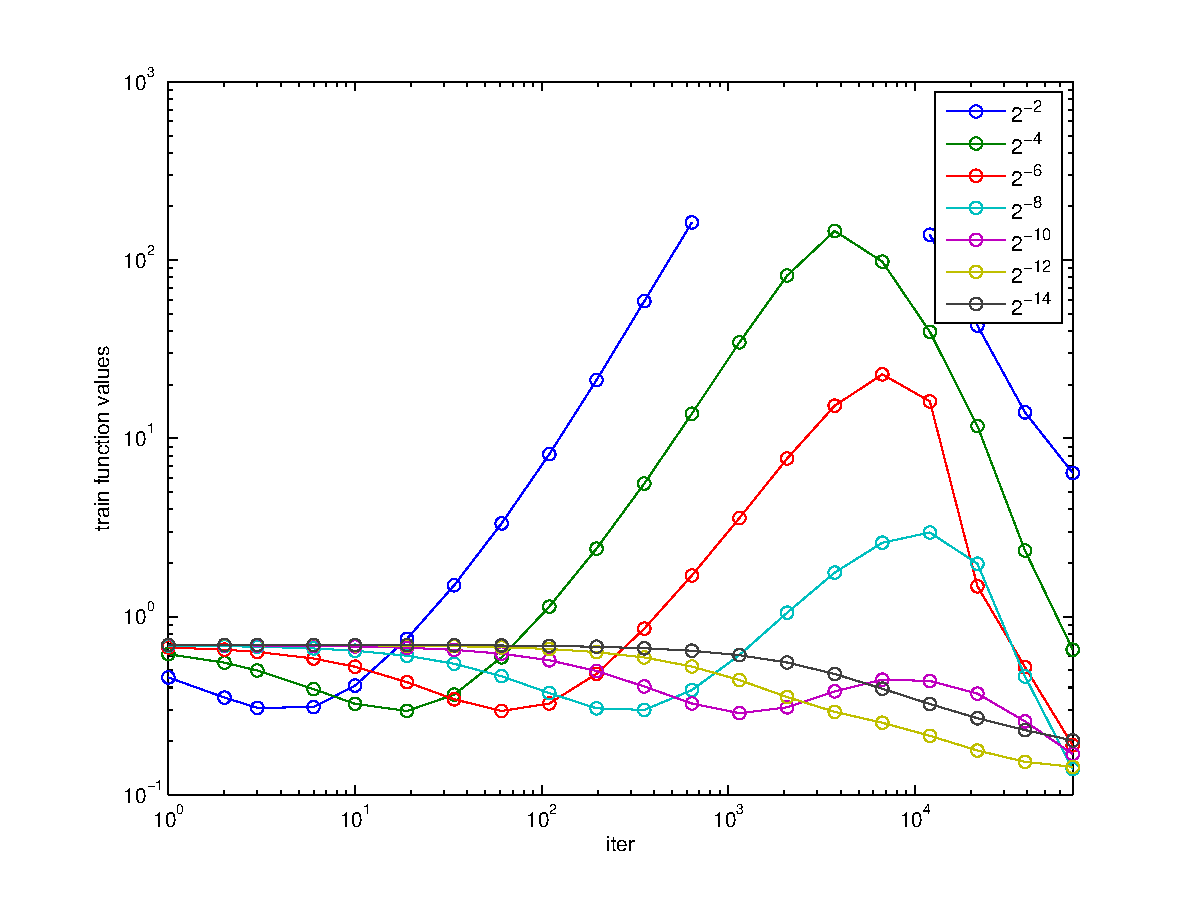
\includegraphics{Figures/sag-log.eps} 
	\end{center}
	\begin{center}
	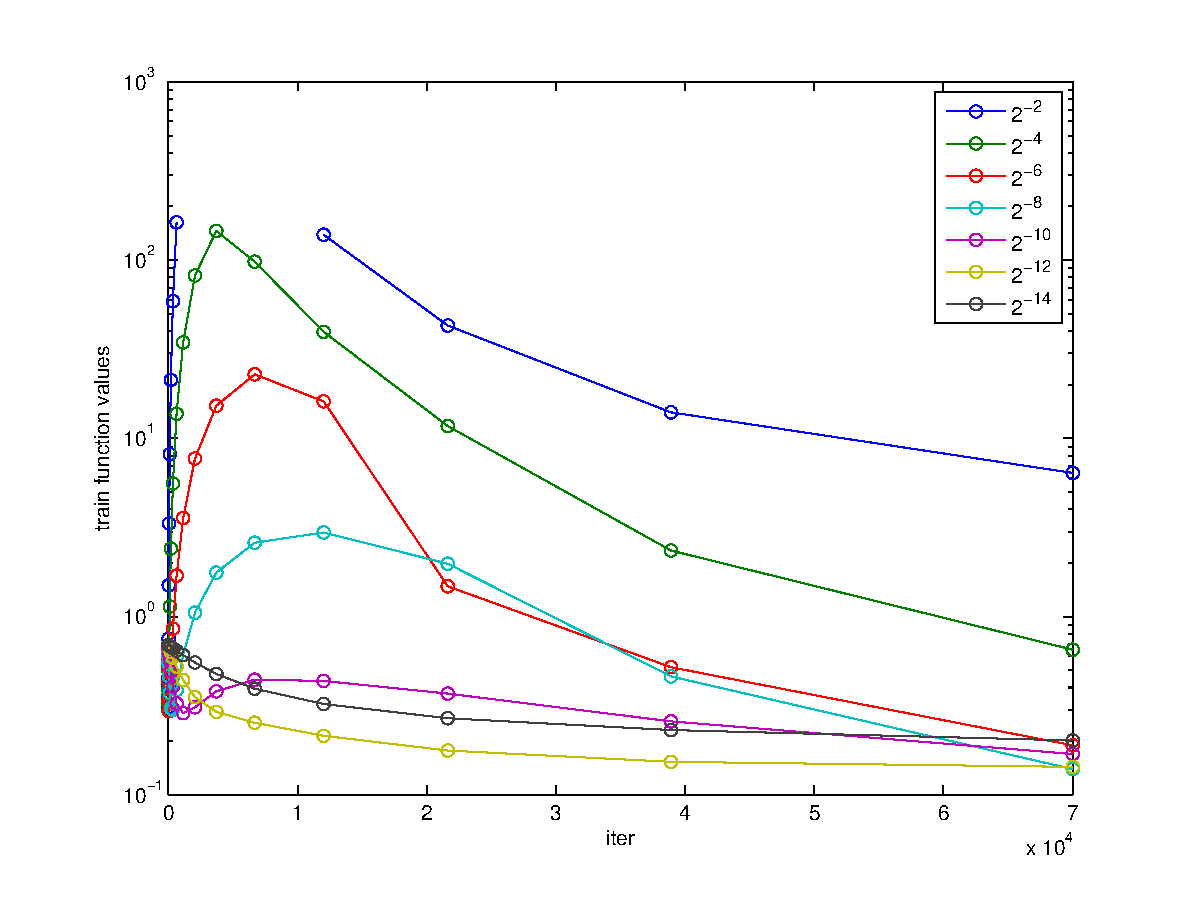
\includegraphics{Figures/sag-nonlog.eps} 
	\end{center}
	\subsection{Compare with reference SAG}
	His choice of steplength $0.006548 \approx 2^{-7}$ and computed by 
	\begin{verbatim}
		Lmax = .25*max(sum(X.^2,2)) + lambda;
		stepSize = 1/Lmax;
		\end{verbatim} 
		
		This SAG variant initialization seems to be different from our framework, since sampling is done at randomly from either set. 
	
	
	\subsection{Larger numerical tests}
	Same random logistic, but now 700000 training points. This is a variant with truly random sampling with replacement of the $S_k$ indices from the sets $I_k$. The last number in the label is the constant step length parameter used. The number of iterations is equal to half of the number of training points available. So the last three plots correspond to a single full pass over the data. 
	
	Some observations can be made: 
	\begin{itemize}
		\item With a large step parameter, good function values are reached initially, but high accuracy is not reached. \\
		\item There is a drastic difference between the two sampling strategies (namely between (1,1) and (0,2)). For all three step choices, (0,2) seems to be doing better initially, but always get taken over by (1,1) when high accuracy is required! This is good news. 
	\end{itemize}

	\begin{center}
	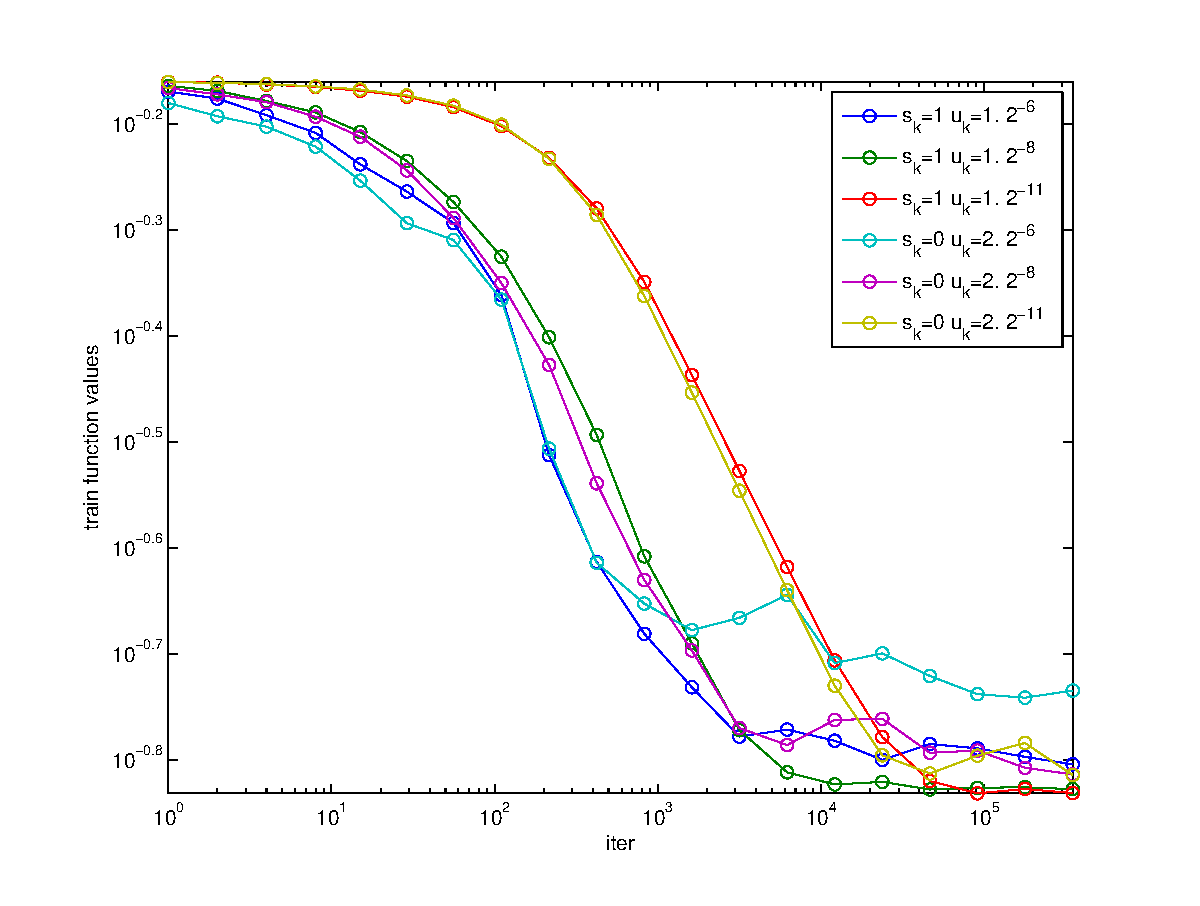
\includegraphics{Figures/12-4.eps}    
	\end{center}

	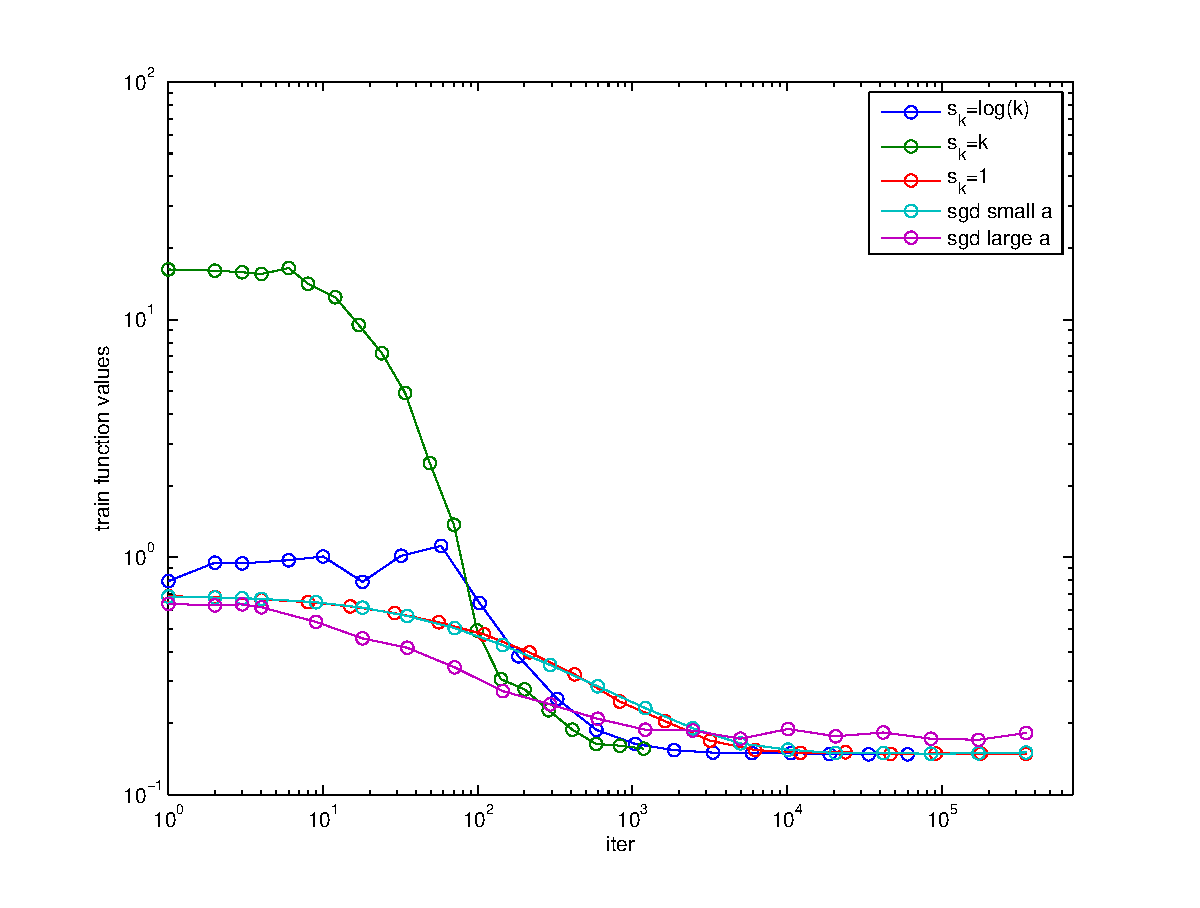
\includegraphics{Figures/12-7-iter.eps}
	
	\includegraphics{Figures/12-7-adp.eps}    
	\subsection{Alpha}
	This is a binary classification problem, and we again use regularized logistic regression. This is a dense problem, with 175000 training points and 501 variables. 
	
	\begin{center}
	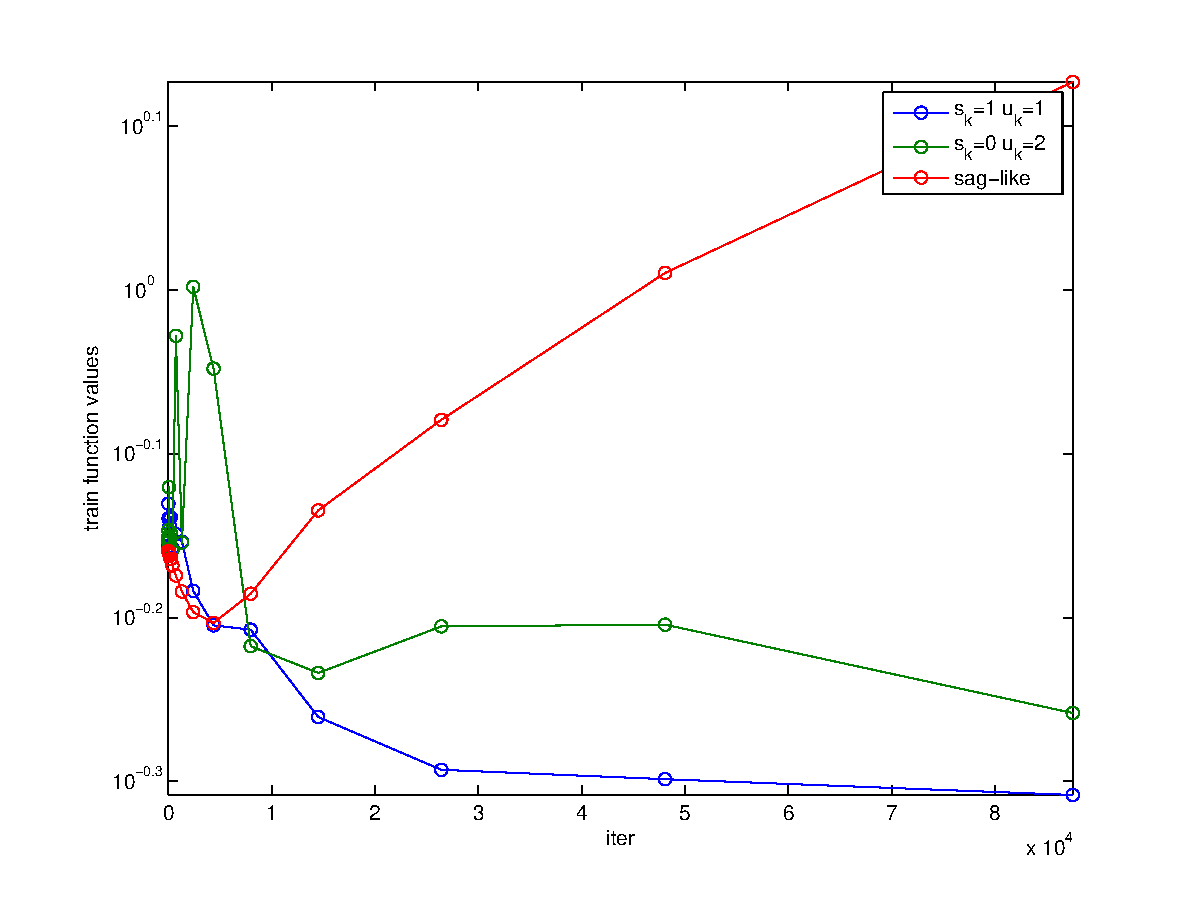
\includegraphics{Figures/12-5.eps}    
	\end{center}
	
	\subsection{Speech Dataset}
	
	We ran the ssag algorithm for one epoch-equivalent, and can observe in the plot below that repeating datapoints is extremely useful. The second plot suggests that repeating must me done at random, and not sequentially. For computational efficiency reasons, along with sampling randomly from $I_k$, we have an option of sampling sequentially, and that is the CHEAP option. Training points: 143706, 30315 variables. 
	
	
	\begin{center}
	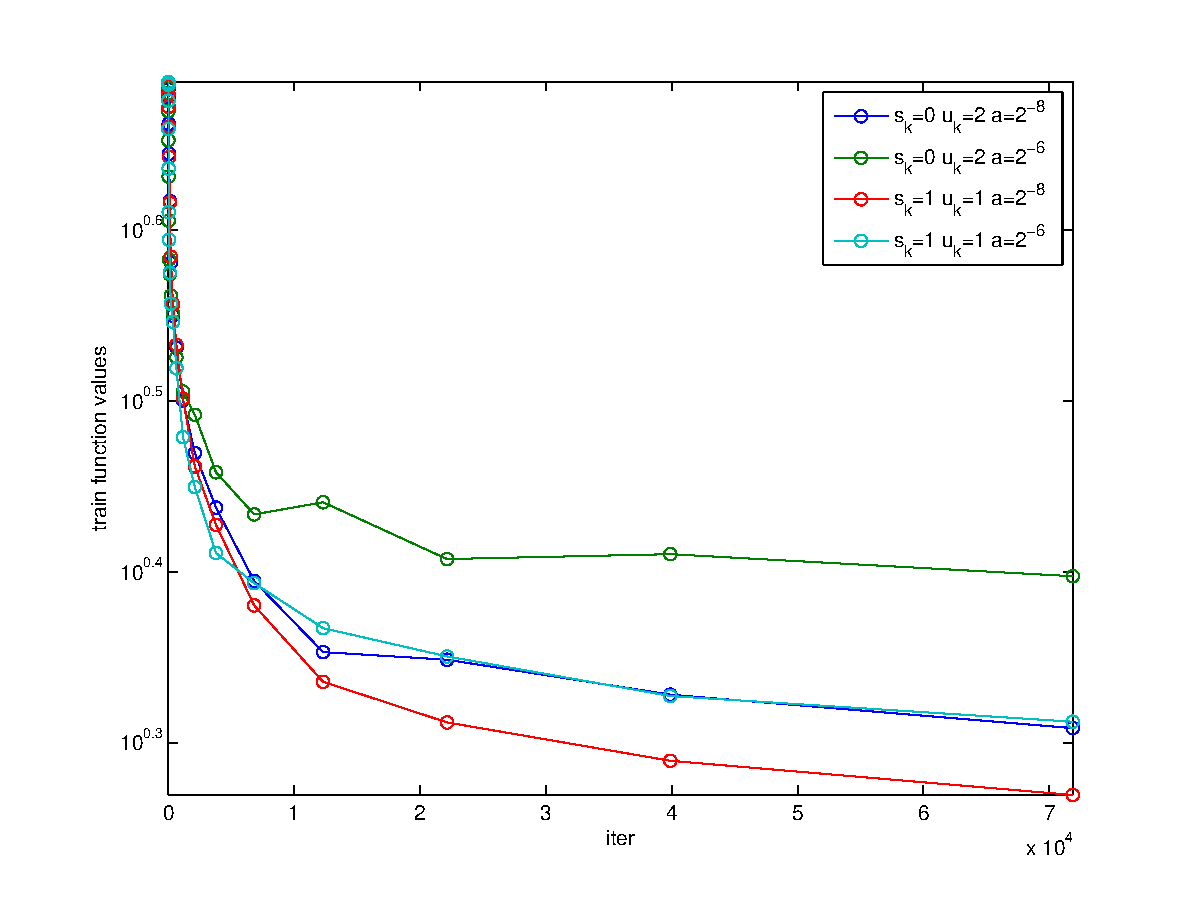
\includegraphics{Figures/12-6.eps}    
	\end{center}

	\begin{center}
	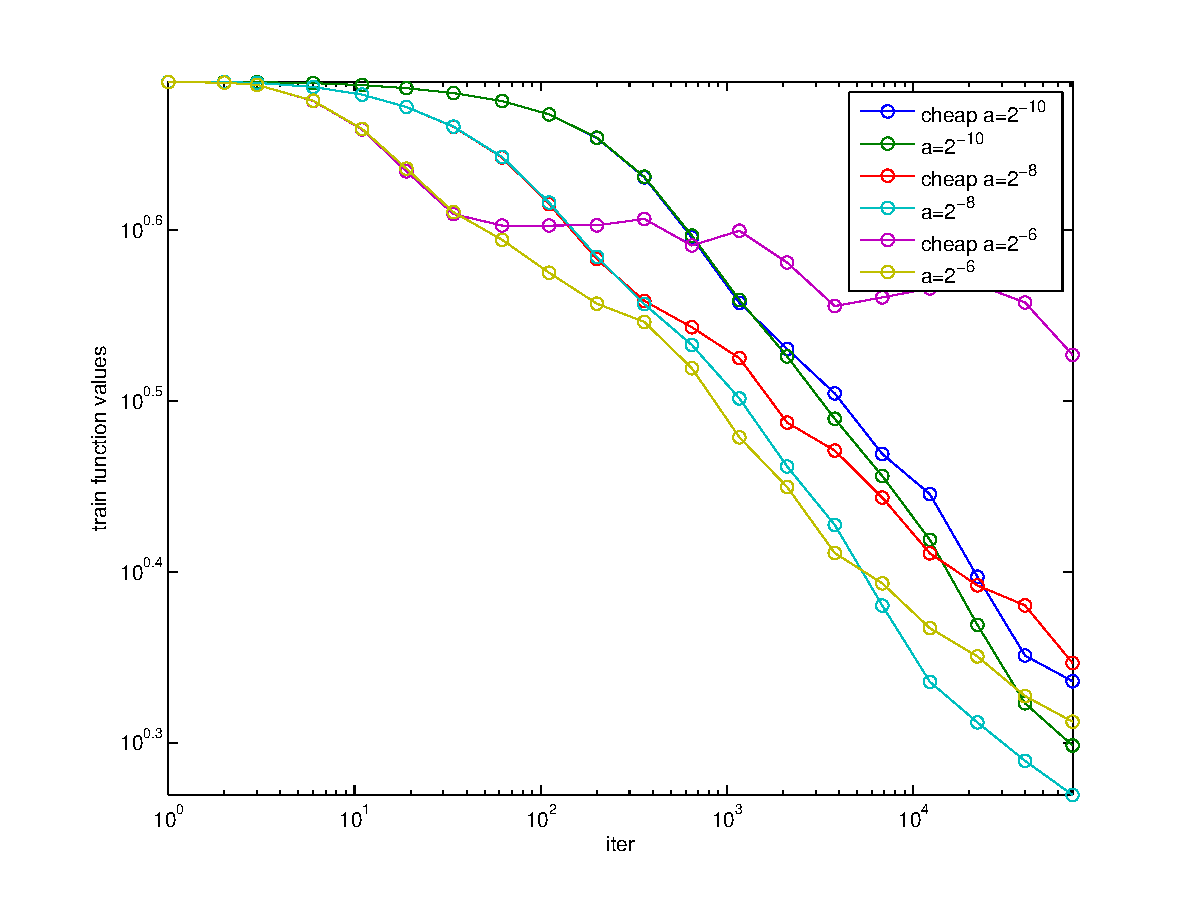
\includegraphics{Figures/12-6-cheap.eps}    
	\end{center}
	
	\section{Large Random Binary Logistic Regression}
	
	This test was conducted on the random logisitic regression problem (Yoram) with L2 regularization parameter $\gamma = 10^{-2}$. 50 variables, 700000 training datapoints. The relative error in the gradient computed by the formula:
	\begin{verbatim}
		norm(ye{1,i}.results.expensiveresults.gradients(:,j) - ye{1,i}.results.expensiveresults.stepDirection(:,j))/norm(ye{1,i}.results.expensiveresults.gradients(:,j))
	\end{verbatim}
	
	\begin{center}
	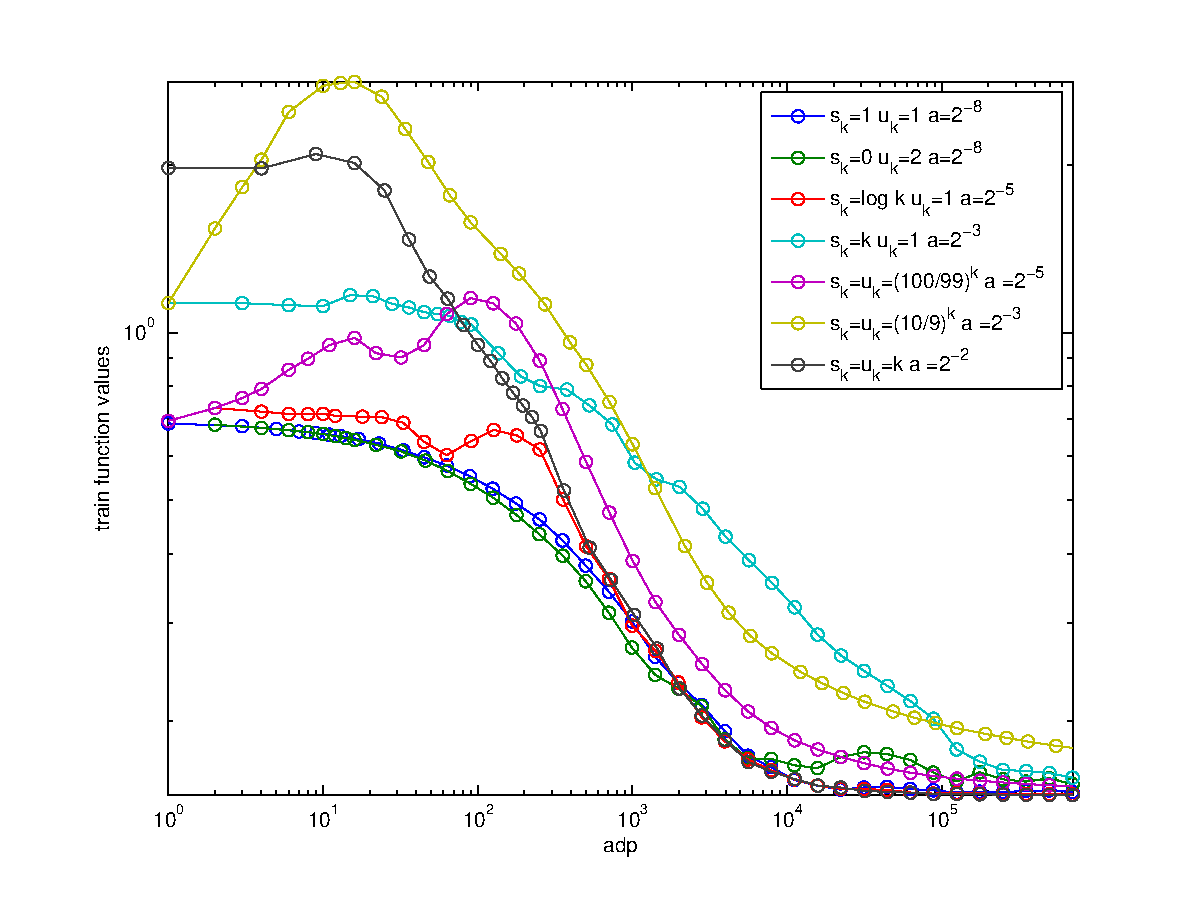
\includegraphics{Figures/LRadp.eps}    
	\end{center}
	
	
	\begin{center}
	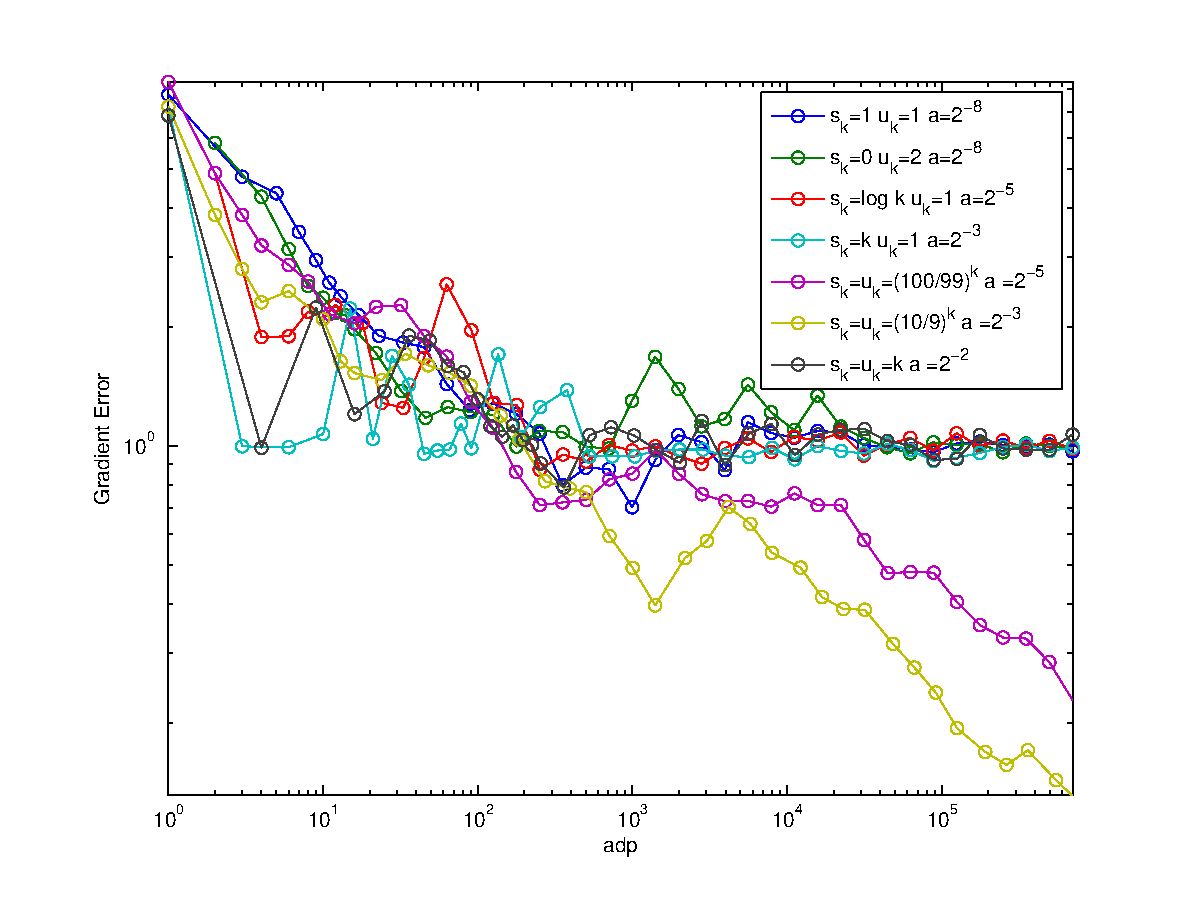
\includegraphics{Figures/LRerror.eps}    
	\end{center}
	
	\begin{center}
	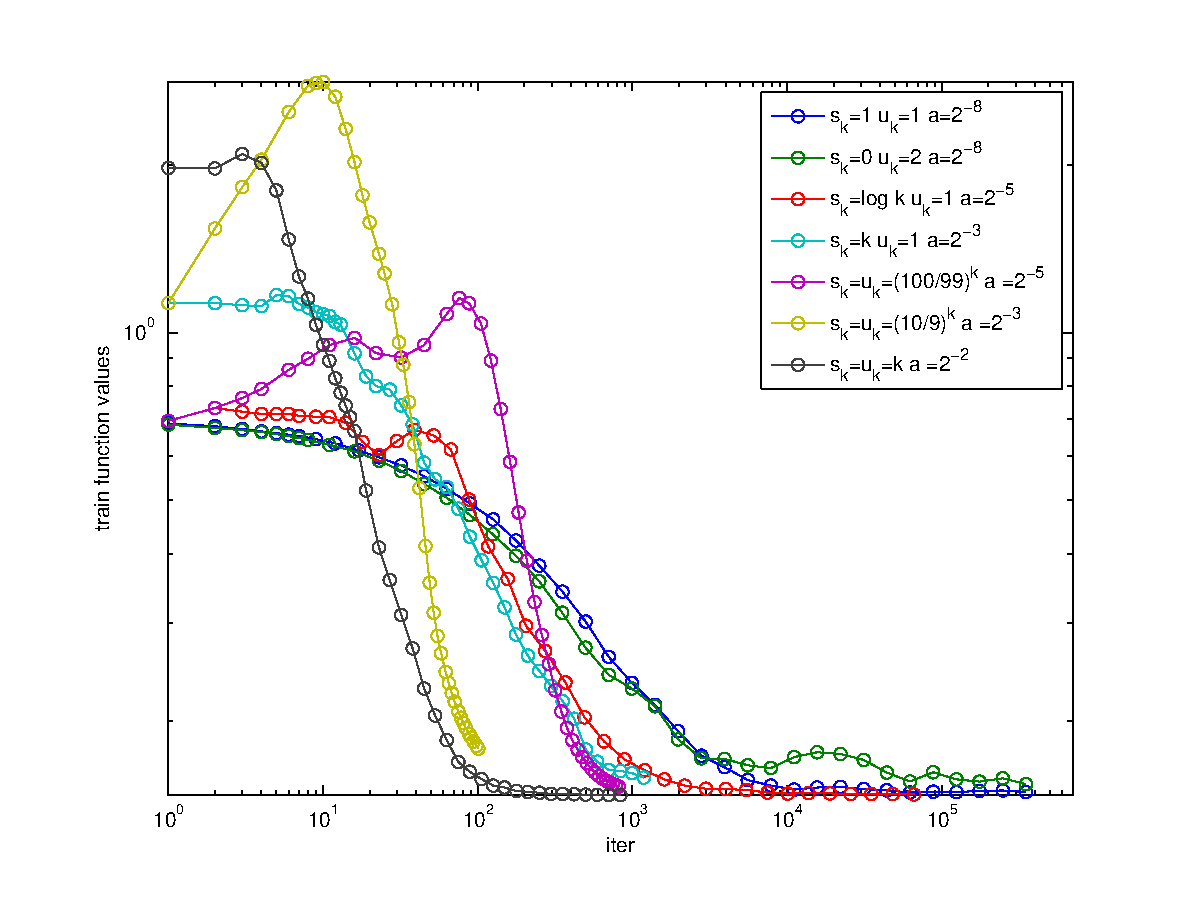
\includegraphics{Figures/LRiter.eps}    
	\end{center}
	
	\newpage
	
	\section{Growth Rates}
	
	Always have that $I_0 = \emptyset$. This means that $s_0=0$, and $u_0>0$. $|I_1| = u_0$, $|I_2 |= u_0+u_1$, and in general $|I_k| = \sum_{i=0}^{k-1} u_i$ for $k>0$.
	
	\begin{center}
	\begin{tabular}{ c|c|c|c|c }
		$u_k$ & $|I_k|$ &  $\frac{u_k}{|I_k|}$ &$s_k \leq |I_k|$ & $\frac{s_k}{|I_k|}$ \\
		\hline
		$2$ & $2k$ & $\frac{1}{k}$&$0$ & $0$ \\
		\hline
		 $1$ & $k$ & $\frac{1}{k}$ &$\min{k,1}$ &$\frac{1}{k}$\\
		\hline
		 $1$ & $k$ & $\frac{1}{k}$&$\log{(k+1)}$ &$\frac{\log{(k+1)}}{k}$ \\
		\hline
		 $1$ & $k$ & $\frac{1}{k}$&$k$ &$1$ \\
		\hline		
		$\begin{array}{ll}c(r-1) & \mbox{ when $k=0$} \\ c\left(\frac{r}{r-1}\right)^{k-1} & \mbox{ when $k>0$}\end{array} $& $cr \left(\frac{r}{r-1}\right)^{k-2}$ & $\frac{1}{r-1}$&$\begin{array}{ll}0 & \mbox{ when $k=0$} \\ c\left(\frac{r}{r-1}\right)^{k-1} & \mbox{ when $k>0$}\end{array} $ &$\frac{1}{r-1}$ \\	
		\hline		
		$k+1$& $\frac{k(k+1)}{2}$ & $\frac{2}{k}$ &$k$ &$\frac{2}{k+1}$ \\
	\end{tabular}
	\end{center}
	
	Remember that these are not precisely implementable: A floor function is always used in the computation of $s_k$ and $u_k$.
	
	\section{Following Discussion with Jorge on August 1st}
	
	We think there are a few approaches for proving convergence of the ERG method. 
	
	\begin{itemize}
		\item DSS approach. Requires geometric growth of the bath size, gradient approaches the true gradient. \\
		\item SVRG approach. Age of gradient estimates is strictly controlled. \\
		\item SAG approach. Every cycle of n iterates gives linearly convergeent iterates. \\
	\end{itemize}
	
	To imitate the DSS approach, I believe the first analysis must be done on the scheme
	\begin{align*}
		s_k=|I_k| \\
		u_k=c^k
	\end{align*}
	Note that this is DIFFERENT from the original DSS paper, since this is again biased towards datapoints from earlier iterations. 
	
	To imitate the SAG approach, have $u_k=C$ for $k=0$, and $0$ otherwise. $s_k=1$ always. 
	
	We can also try a hybrid SVRG-SAG  step direction, of $\nabla \psi_i (x^k) - \nabla \psi_i (x^{prev}) + g^{SAG}$
	
	\newpage 
	\section{Aug2 Experiments on the Large Random Problem}
	In the following experiments, the steplength parameter is tuned for each method in one of the two ways:
	\begin{enumerate}
		\item Find steplength such that the function value drops beneath the specified value (blue horizontal line) after smallest amount of adp
		\item Find steplength that gives the lowest function value withing the specified adp limit
	\end{enumerate}
	The used parameter is specified in the graph legend.
	
	\newpage
	
	\subsection{Exponential Increase in $s_k=u_k$}
	
	This experiment was conducted to demonstrate the characteristics of the exponential growth rates (5th choice in the Growth Rates table). Here we always set $c=1$, and choose $r$ to give one of the following ratios for $\frac{u_k}{|I_k|}$: $0.1\%, 1\%, 10\%, 50\%, 100\%$. The steplength was tuned to give the lowest training objective value withing the allotted adp limit (1 pass-equivalent).
	
\begin{figure}[H]
\begin{subfigure}[b]{.5\linewidth}
	        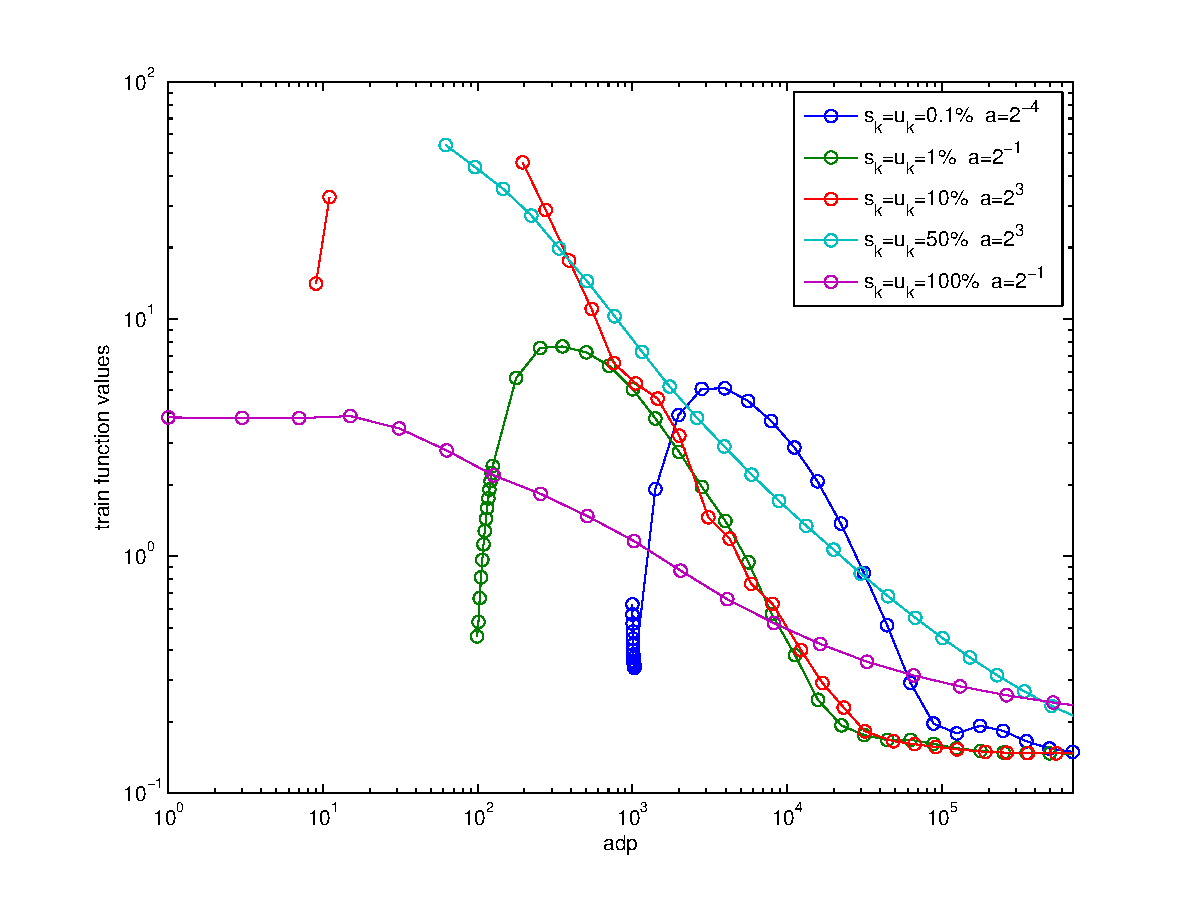
\includegraphics[width=4in]{Figures/exp1.eps}
\end{subfigure}%
\begin{subfigure}[b]{.5\linewidth}
	        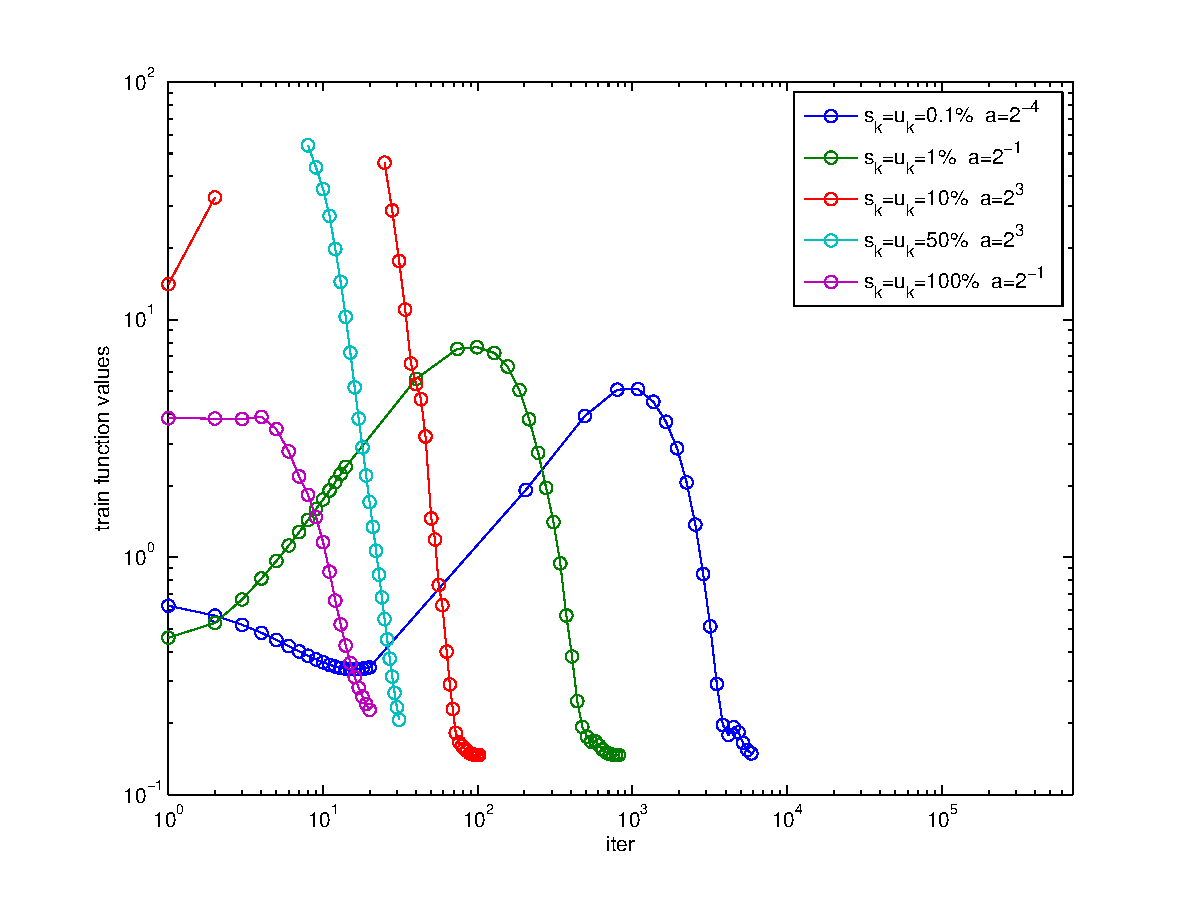
\includegraphics[width=4in]{Figures/exp2.eps}
\end{subfigure}%

\begin{subfigure}[b]{.5\linewidth}
	        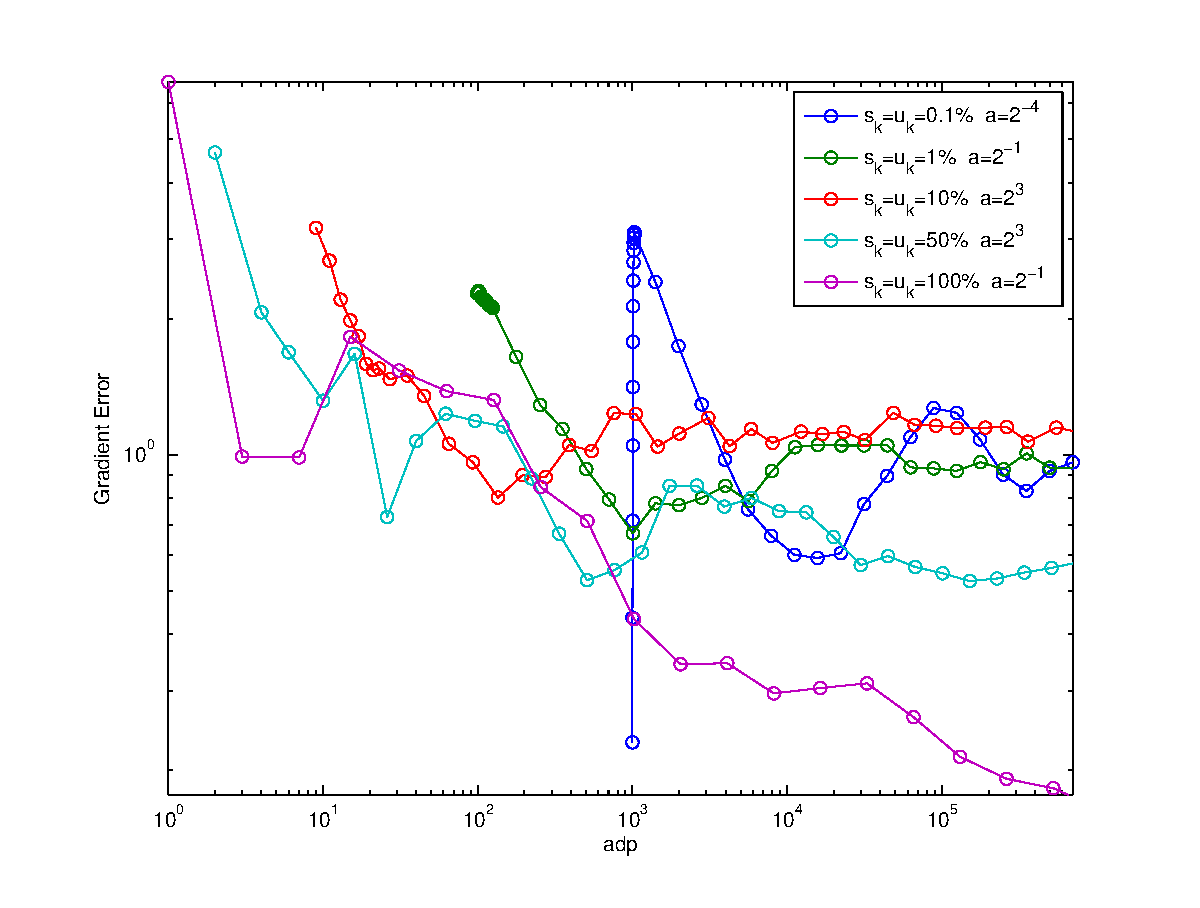
\includegraphics[width=4in]{Figures/exp3.eps}
\end{subfigure}%
\begin{subfigure}[b]{.5\linewidth}
	        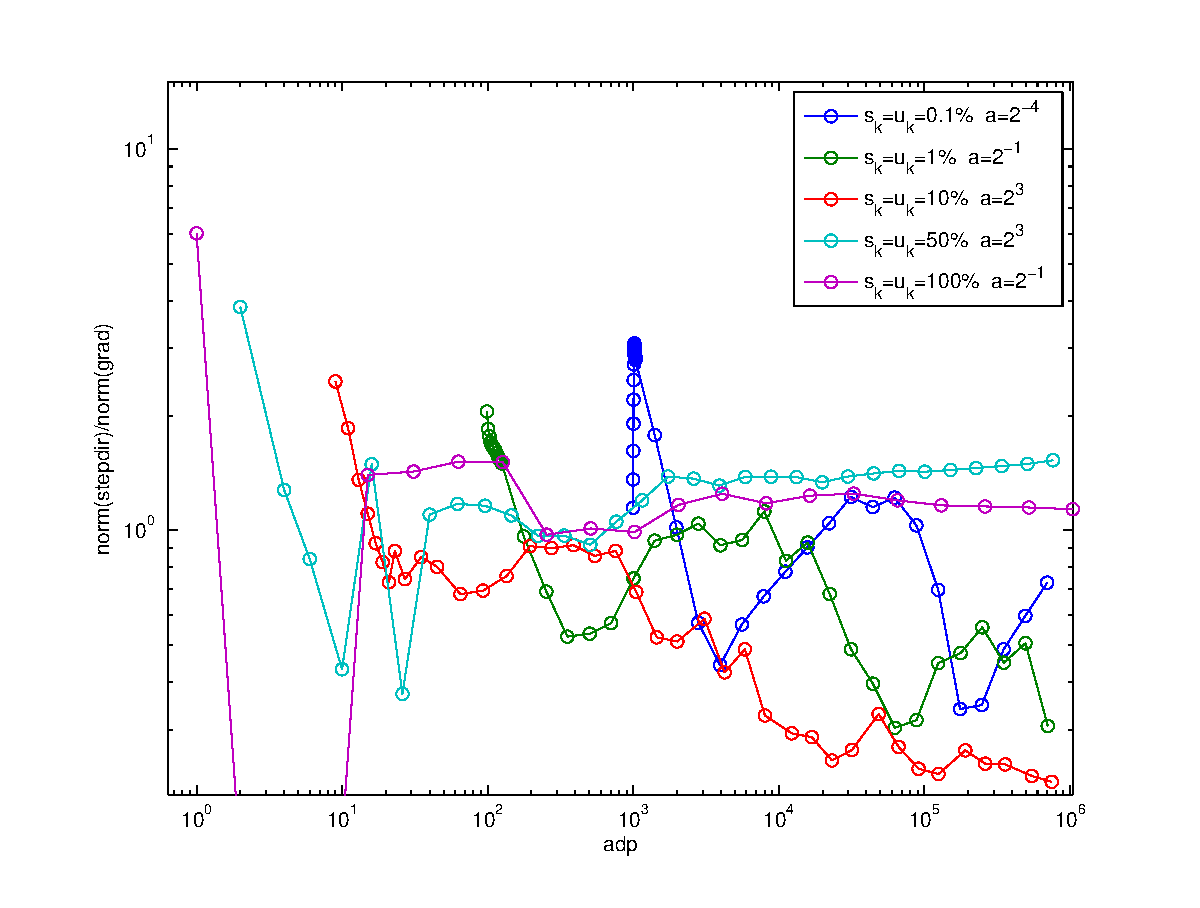
\includegraphics[width=4in]{Figures/exp4.eps}
\end{subfigure}%
\end{figure}

\begin{itemize}
	\item The blue method starts off with a very good gradient, thus the small starting gradient error.
	\item The purple method, seems to attempt working in a deterministic regime right away. Thus the conservative choice of stepsize. This is the only method that gets a reliably good gradient estimate, as can be seen in the gradient error.
	\item Purple and cyan methods are not competetive within the given adp limit because of rapid batch size increase.
\end{itemize}
	\newpage
	The following plots show the same methods, but with steplength parameter chosen to satisfy a different objective: To reach a certain function value the fastest. This line is shown in blue. fValueNeeded=$10^{-0.64}$
	
\begin{figure}[H]
\begin{subfigure}[b]{.5\linewidth}
	        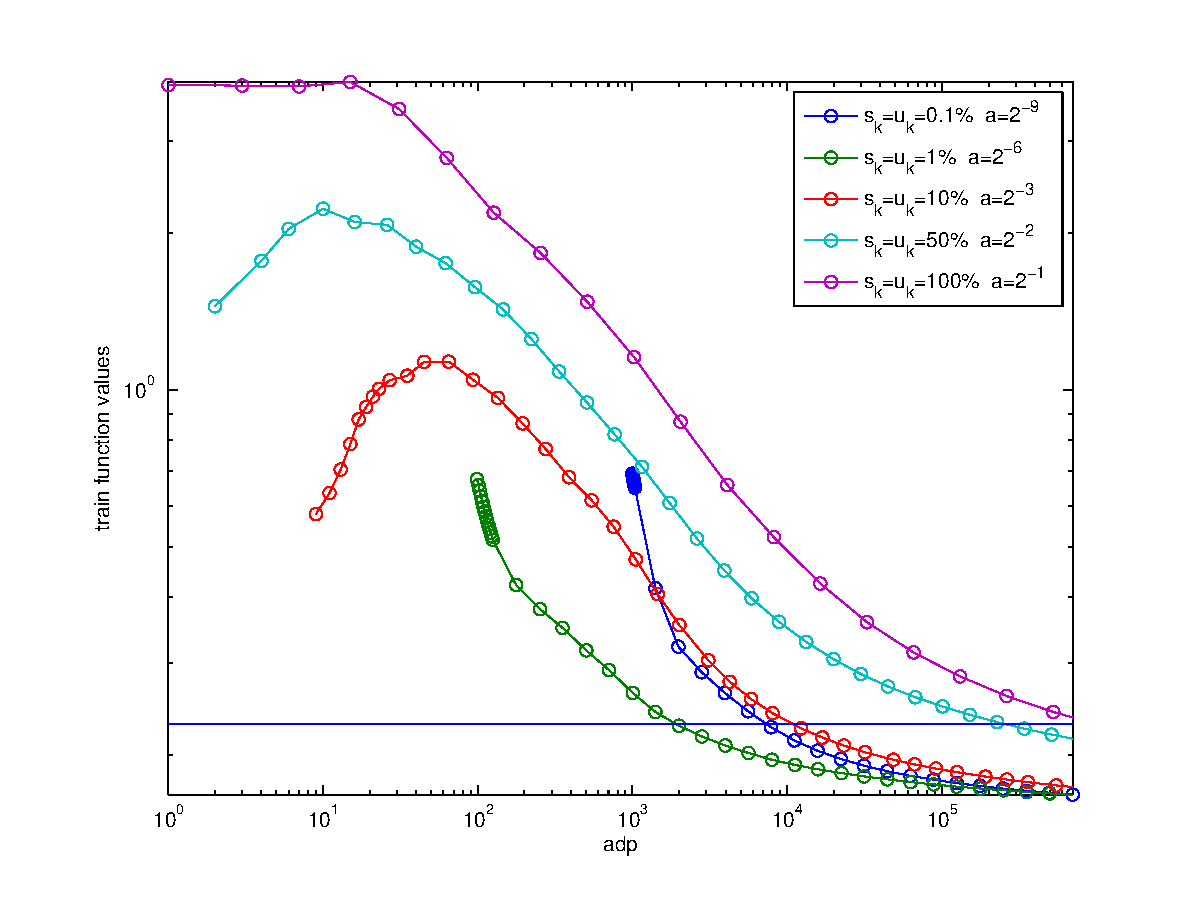
\includegraphics[width=4in]{Figures/exp2-1.eps}
\end{subfigure}%
\begin{subfigure}[b]{.5\linewidth}
	        \includegraphics[width=4in]{Figures/exp2-2.eps}
\end{subfigure}%

\begin{subfigure}[b]{.5\linewidth}
	        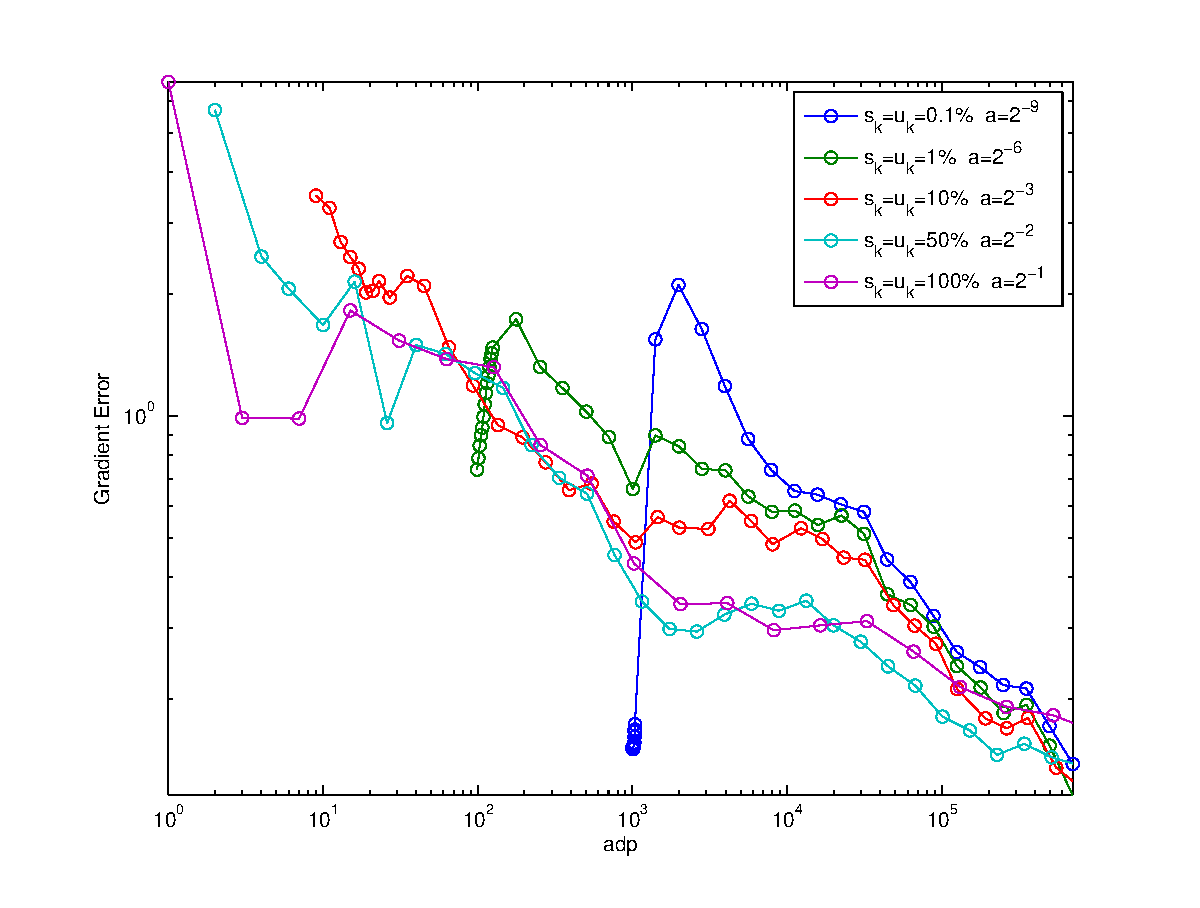
\includegraphics[width=4in]{Figures/exp2-3.eps}
\end{subfigure}%
\begin{subfigure}[b]{.5\linewidth}
	        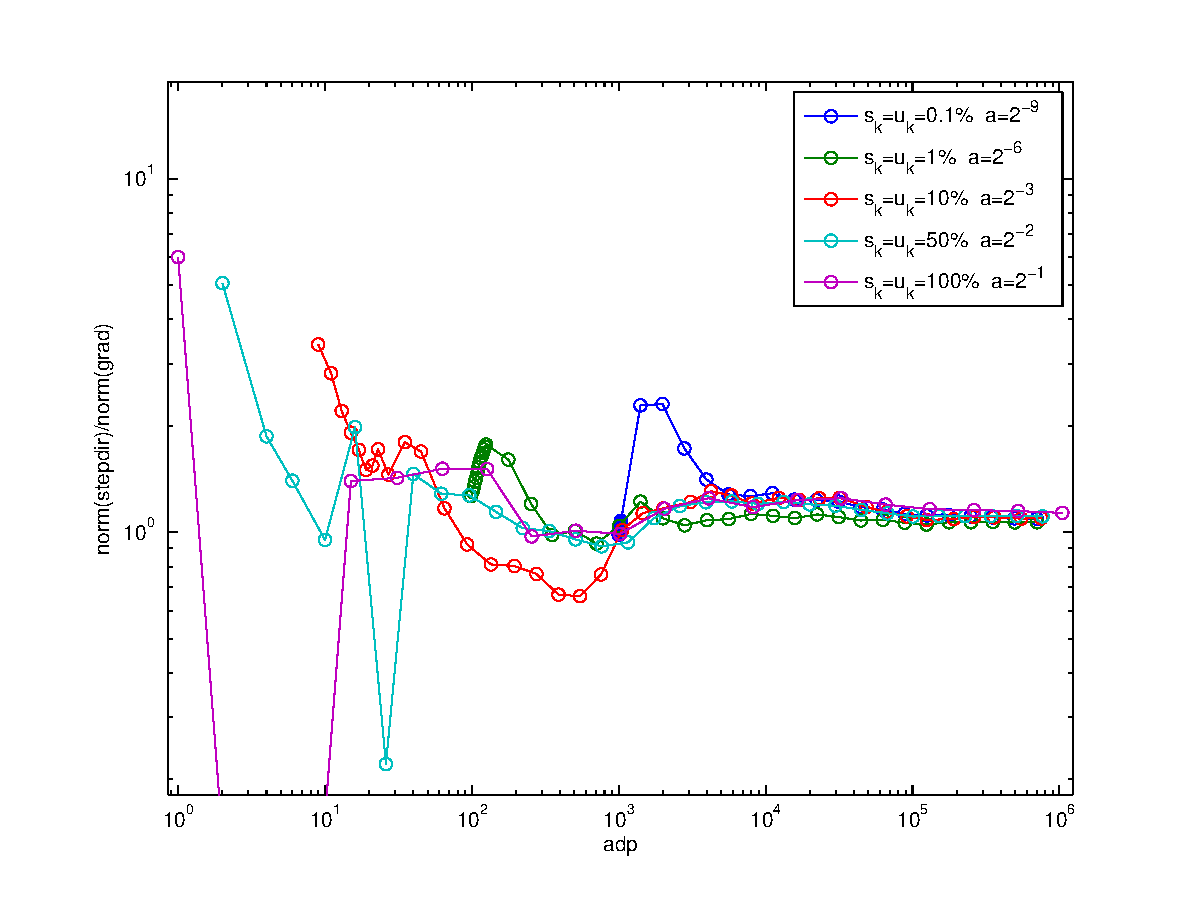
\includegraphics[width=4in]{Figures/exp2-4.eps}
\end{subfigure}%
\end{figure}
	
	Now the steplengths are chosen much more conservatively: the methods attempt to keep old information relevant by not stepping too far. All methods have a substantial tendency to emulate the true gradient.
	
	\newpage
	
	\subsection{Who wins?}
	
	Here we compare a few of the suggested methods, again choosing a step parameter such that the lowest objective value is reached. 
	
	\begin{figure}[H]
	\begin{subfigure}[b]{.5\linewidth}
		        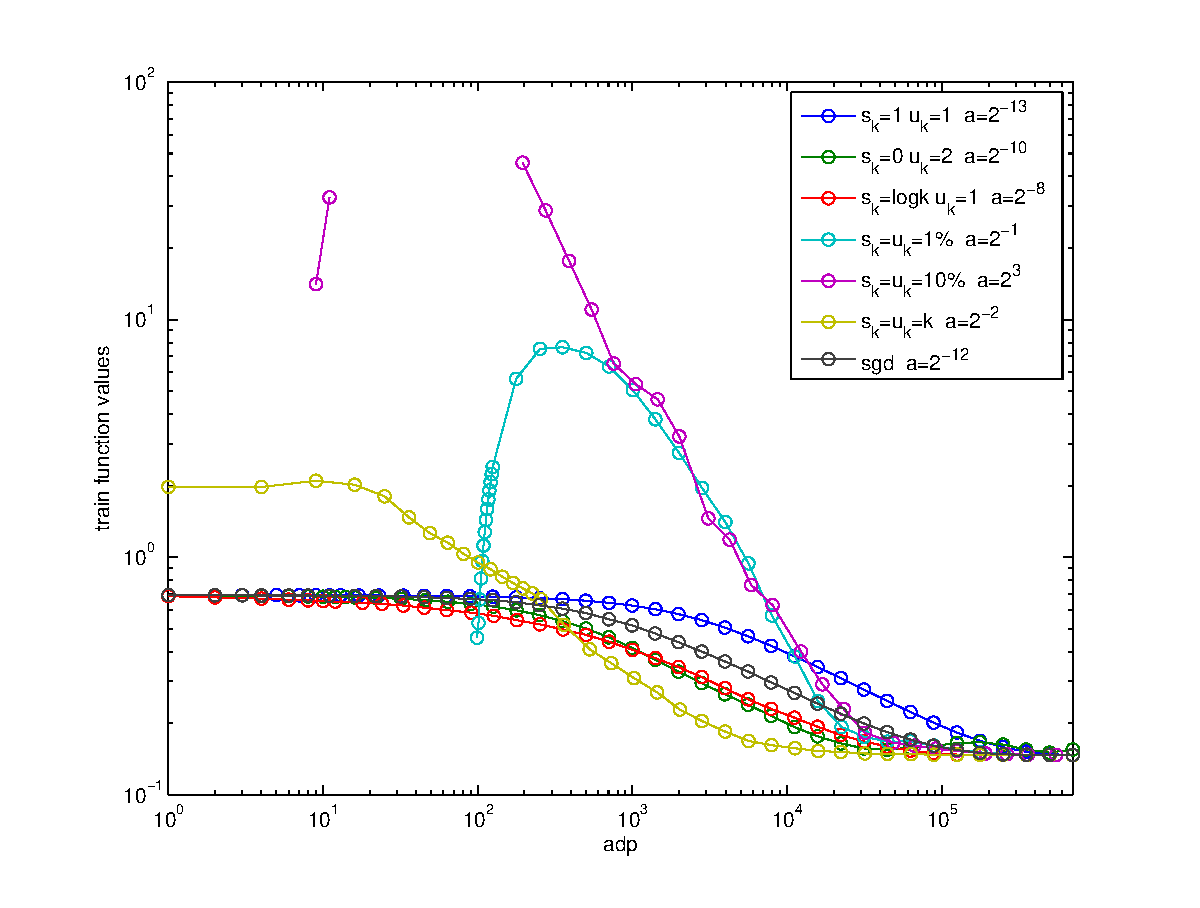
\includegraphics[width=4in]{Figures/whowins1.eps}
	\end{subfigure}%
	\begin{subfigure}[b]{.5\linewidth}
		        \includegraphics[width=4in]{Figures/whowins2.eps}
	\end{subfigure}%

	\begin{subfigure}[b]{.5\linewidth}
		        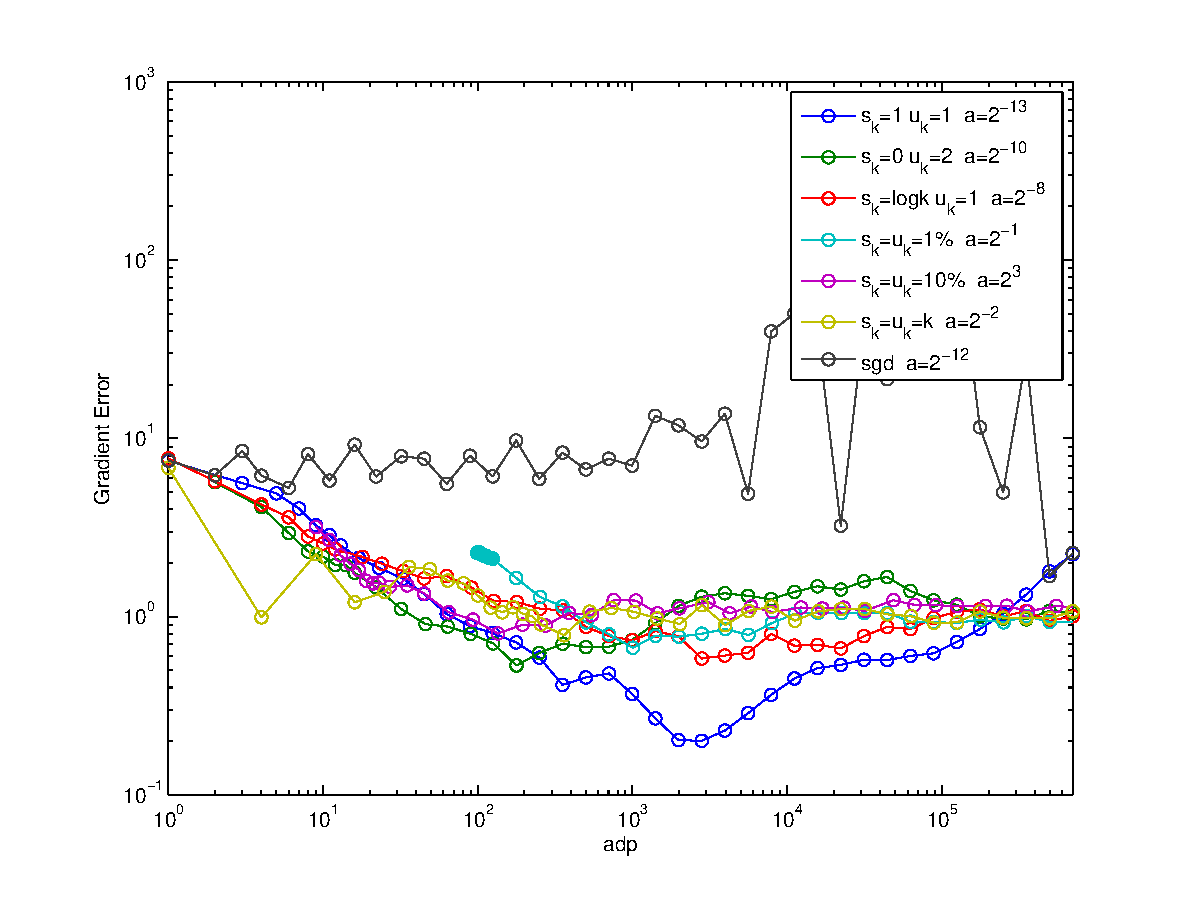
\includegraphics[width=4in]{Figures/whowins3.eps}
	\end{subfigure}%
	\begin{subfigure}[b]{.5\linewidth}
		        \includegraphics[width=4in]{Figures/whowins4.eps}
	\end{subfigure}%
	\end{figure}
	
	
	\begin{itemize}
		\item Unfortunately, there is no clear winner (all except for the green method achieve roughly the same function values).
		\item The fact that the yellow method seems to do well on the adp graph. Other methods don't look as good, but they have a different objective: to reach the best function value they can, not to look the best at some intermediate stage. 
		\item SGD error behaves erratically, as expected
	\end{itemize}
	
	\newpage
	
	If the same methods are asked to reach an intermediate function value, a different picture emerges. fValueNeeded=$10^{-0.82}$;
	
	\begin{figure}[H]
	\begin{subfigure}[b]{.5\linewidth}
		        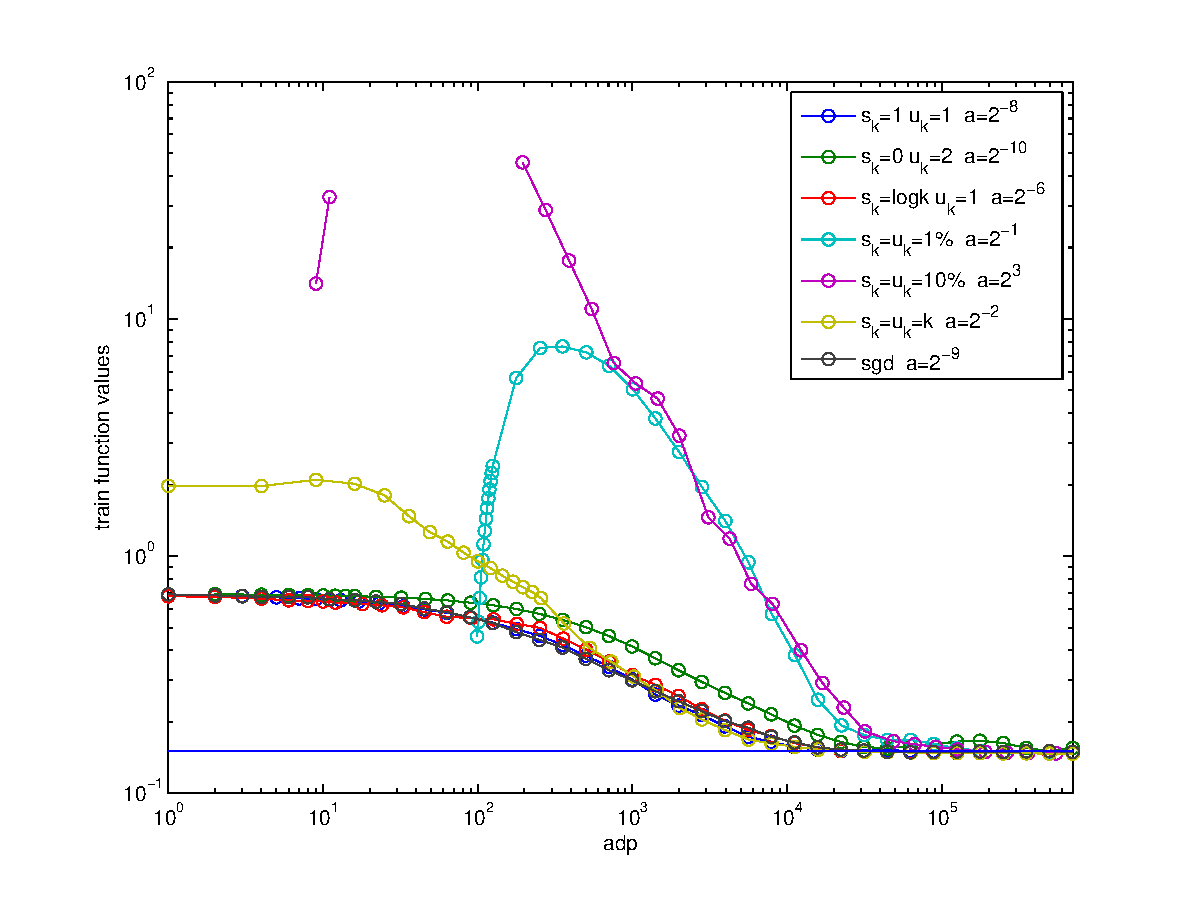
\includegraphics[width=4in]{Figures/whowins2-1.eps}
	\end{subfigure}%
	\begin{subfigure}[b]{.5\linewidth}
		        \includegraphics[width=4in]{Figures/whowins2-2.eps}
	\end{subfigure}%

	\begin{subfigure}[b]{.5\linewidth}
		        \includegraphics[width=4in]{Figures/whowins2-3.eps}
	\end{subfigure}%
	\begin{subfigure}[b]{.5\linewidth}
		        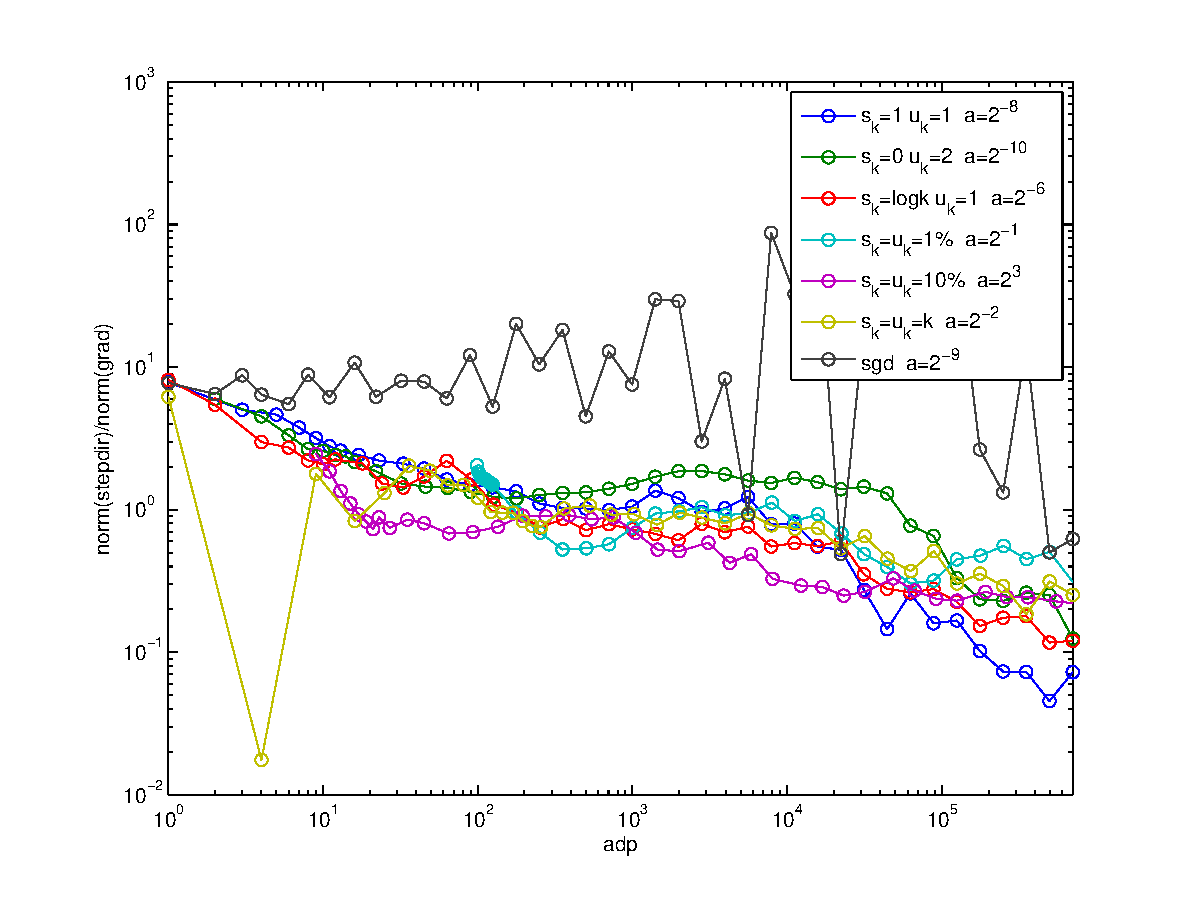
\includegraphics[width=4in]{Figures/whowins2-4.eps}
	\end{subfigure}%
	\end{figure}
	
	\begin{itemize}
		\item The steplength parameters of all methods except for the exponential ones and the yellow one have increased significantly. 
		\item There are clear losers here, even though they are not distinguishable on the top left plot. The exponential methods and the green one require significantly more effort to reach the required function value. 
	\end{itemize}
	
	\newpage
	
	Finally, if we require attaining only a modest function value, fValueNeeded=$10^{-0.64}$, the one used in section 16-1, we observe yet another pattern. 
	
	\begin{figure}[H]
	\begin{subfigure}[b]{.5\linewidth}
		        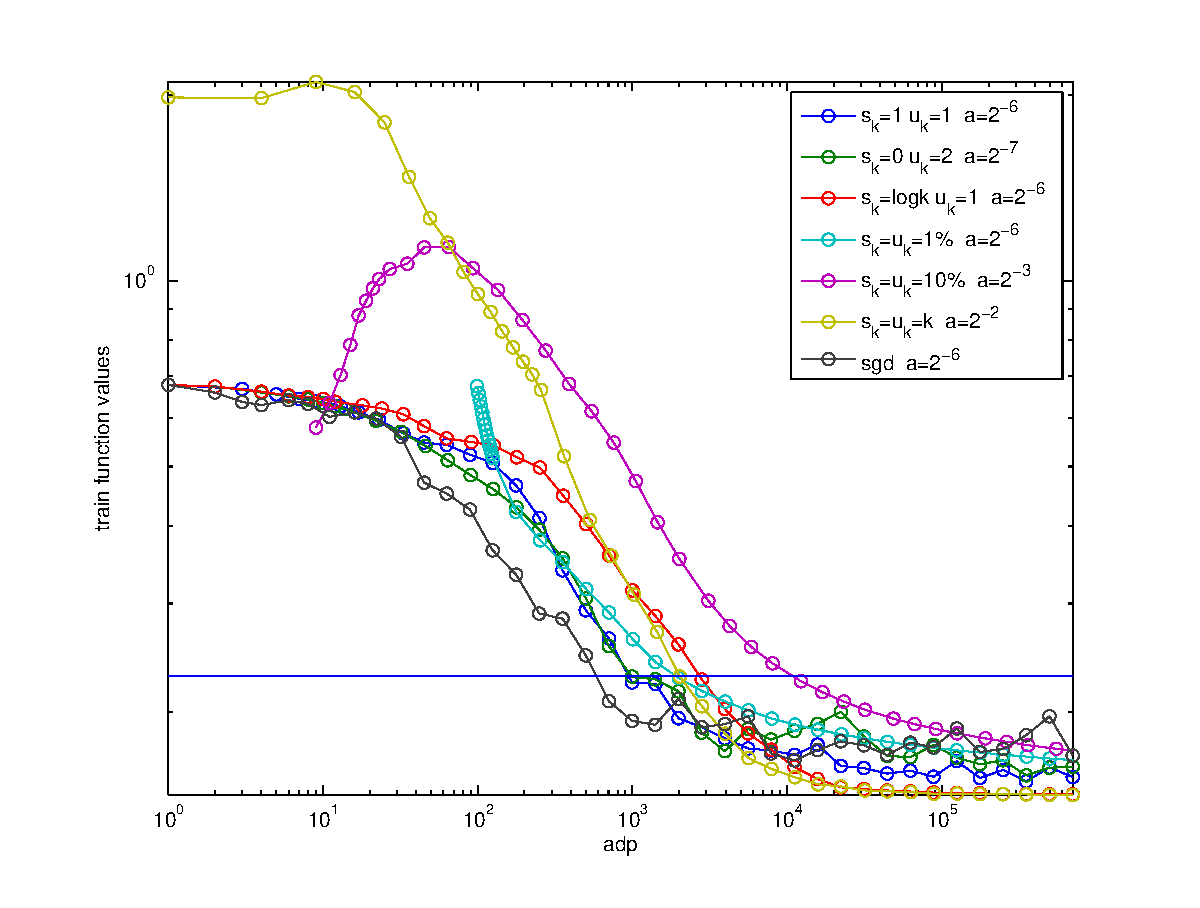
\includegraphics[width=4in]{Figures/whowins3-1.eps}
	\end{subfigure}%
	\begin{subfigure}[b]{.5\linewidth}
		        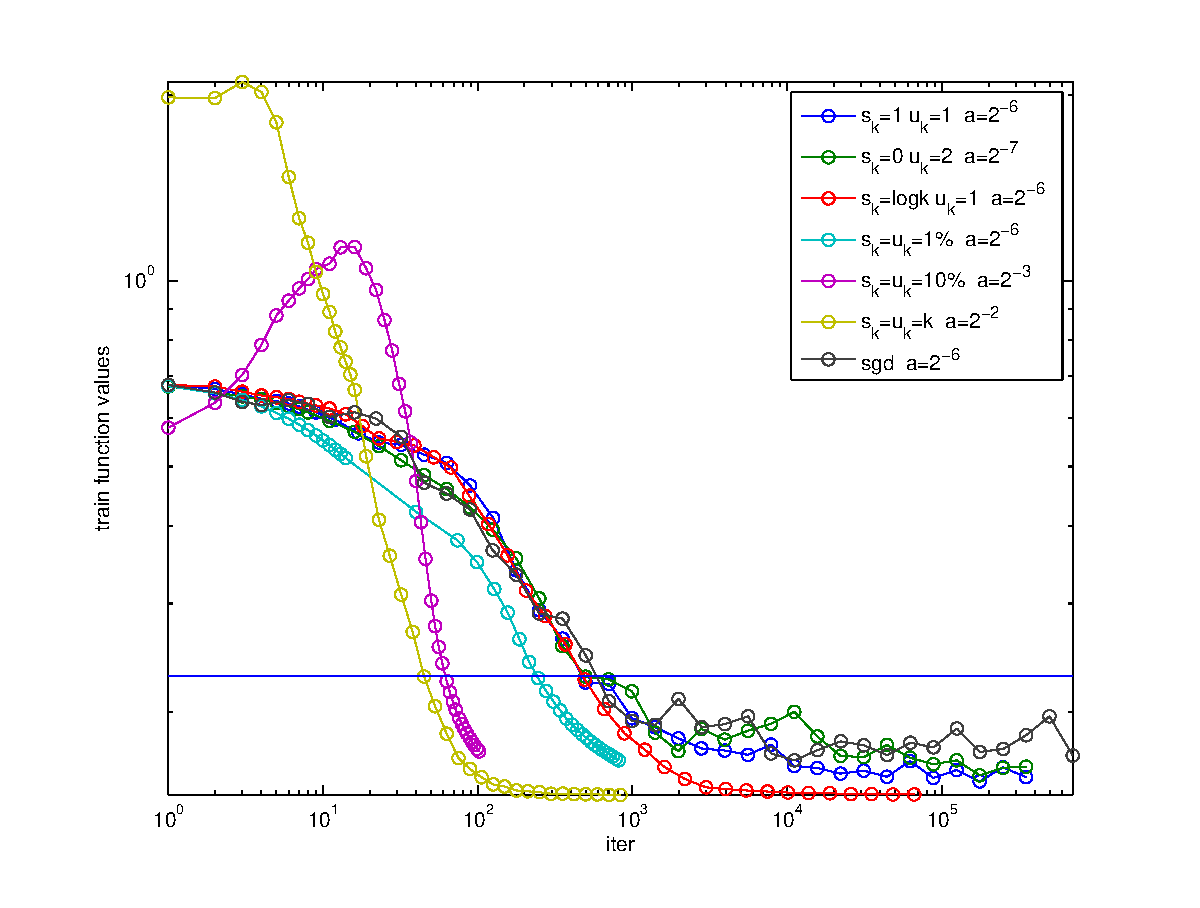
\includegraphics[width=4in]{Figures/whowins3-2.eps}
	\end{subfigure}%

	\begin{subfigure}[b]{.5\linewidth}
		        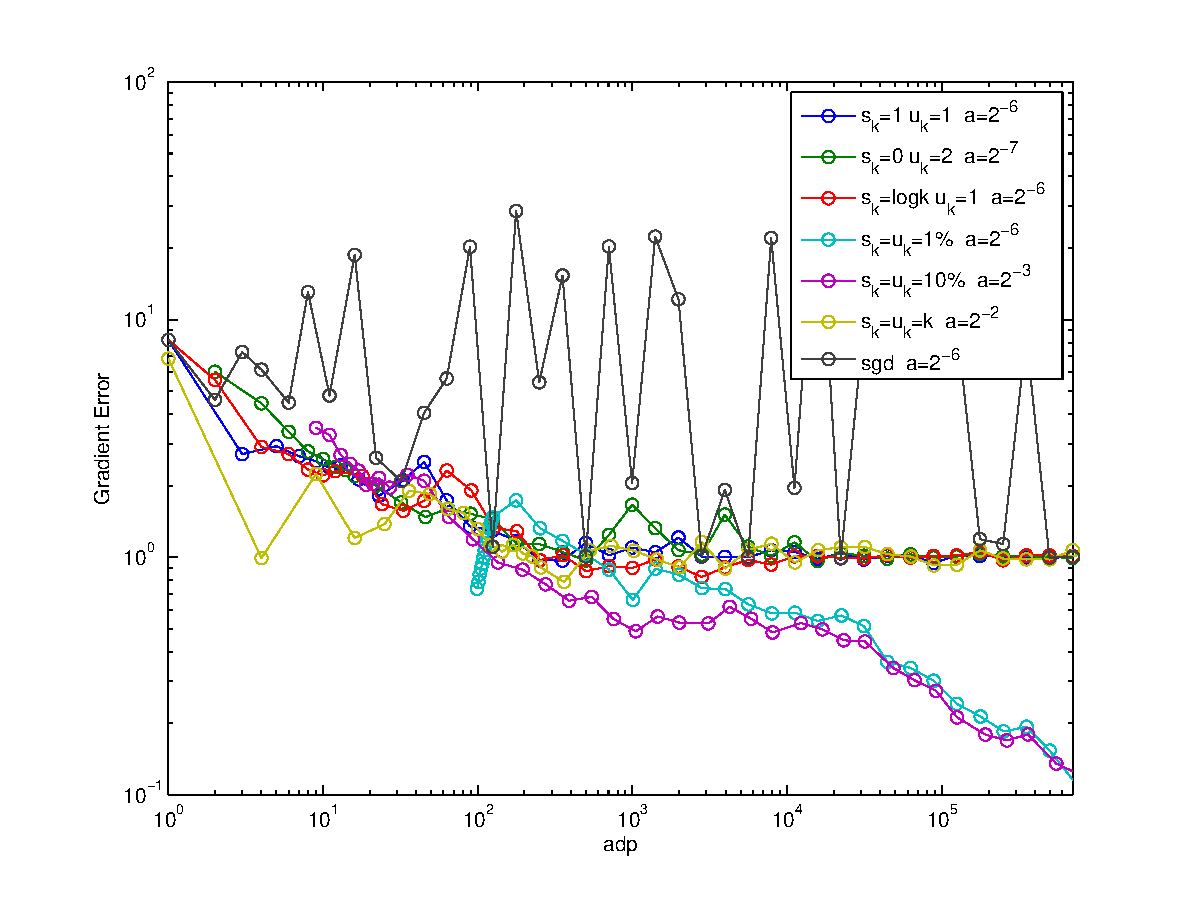
\includegraphics[width=4in]{Figures/whowins3-3.eps}
	\end{subfigure}%
	\begin{subfigure}[b]{.5\linewidth}
		        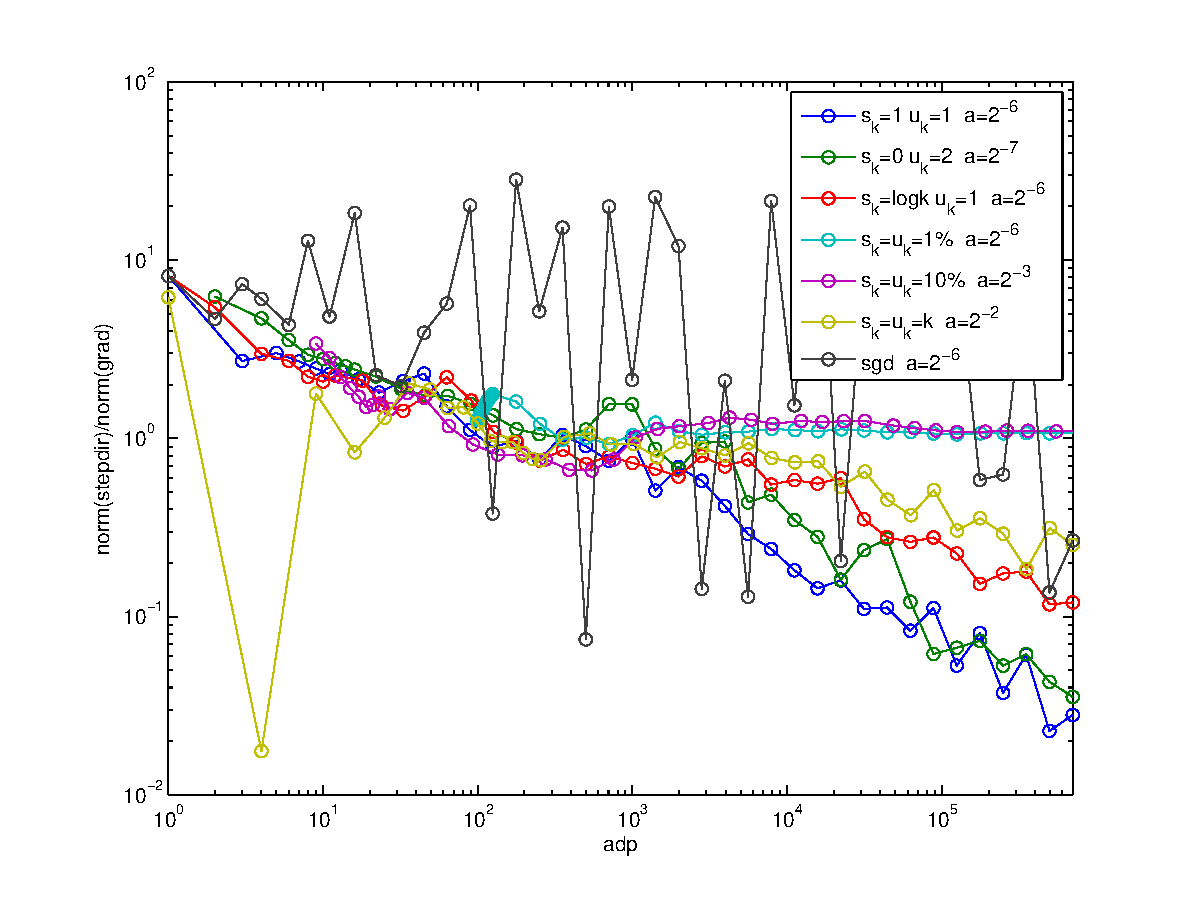
\includegraphics[width=4in]{Figures/whowins3-4.eps}
	\end{subfigure}%
	\end{figure}
	
	\begin{itemize}
		\item Majestically (a keen obeserver might proclaim) the optimal steplength parameter for the yellow method has been constant throughout the three previous experiements! The same method, without special parameter tuning was competetive when used for completely different purposes. This cannot be said of SGD: a method that performed well in the experiments, but required a different step parameter. 
	\end{itemize}
	
	\newpage
	
	\subsection{Now Same problem run for 5 passes over data}
	Sorry, the green method is different, but the rest are the same. Again, we tune to give the lowest function value. Here if the data is exhausted, the corresponding sequence is set to zero in case of $u_k$ and to $\|I_k\|$ in case of $s_k$
	
	
	\begin{figure}[H]
	\begin{subfigure}[b]{.5\linewidth}
		        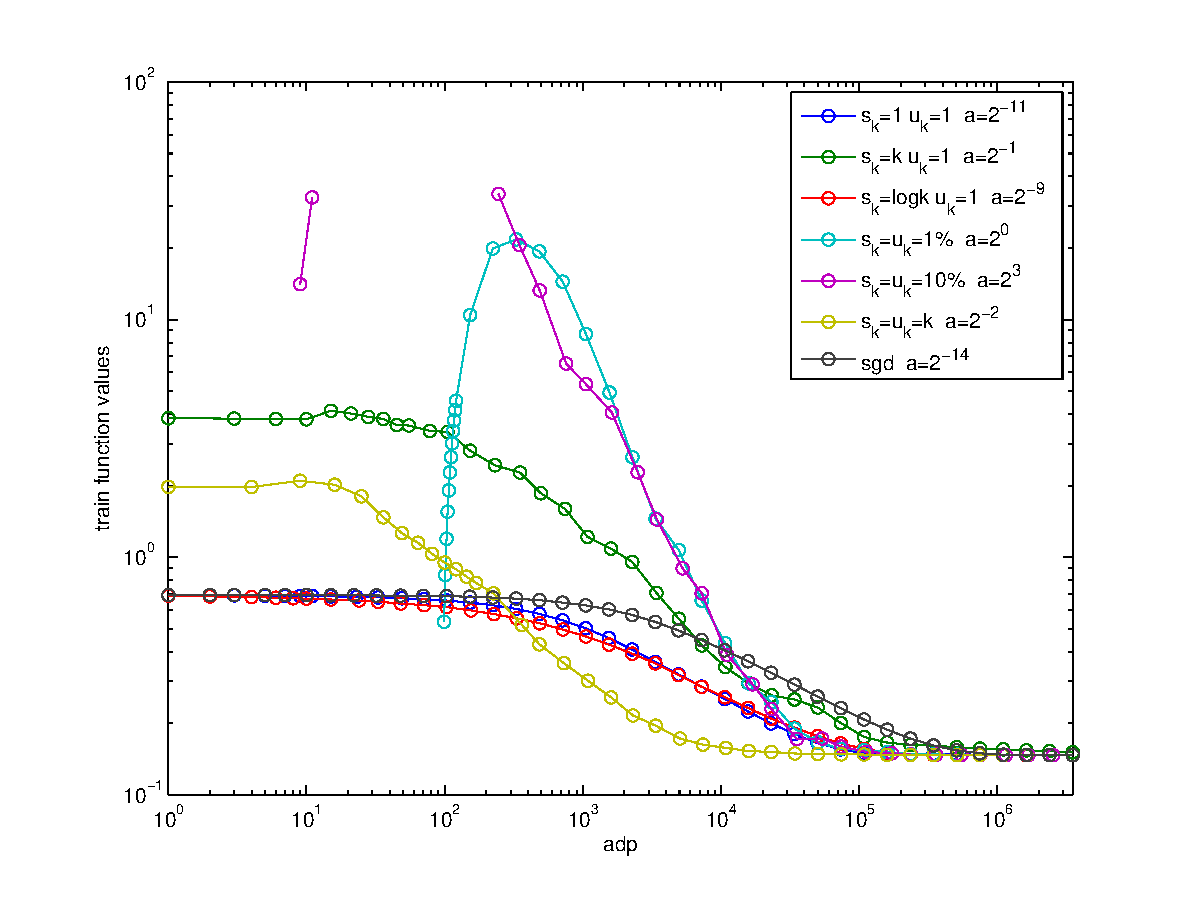
\includegraphics[width=4in]{Figures/16-3-1.eps}
	\end{subfigure}%
	\begin{subfigure}[b]{.5\linewidth}
		        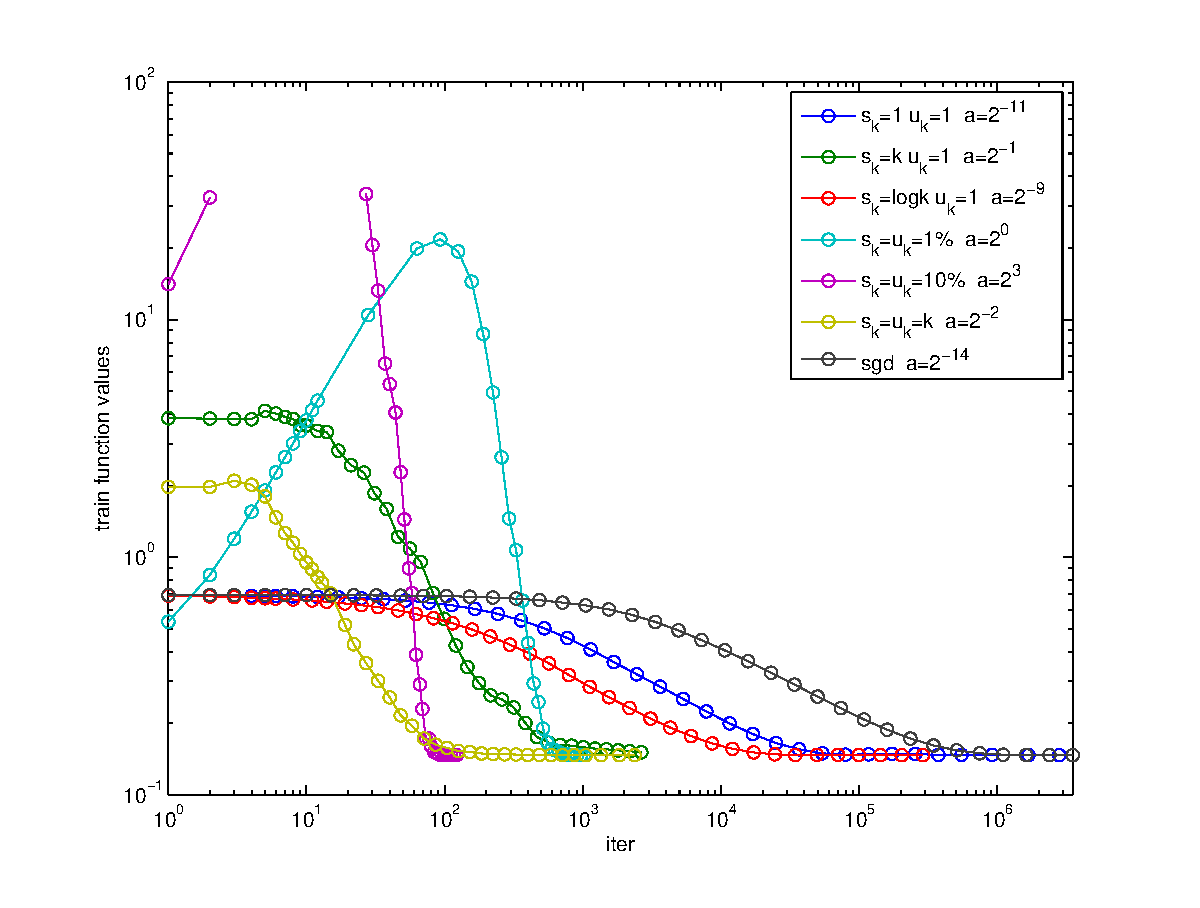
\includegraphics[width=4in]{Figures/16-3-2.eps}
	\end{subfigure}%

	\begin{subfigure}[b]{.5\linewidth}
		        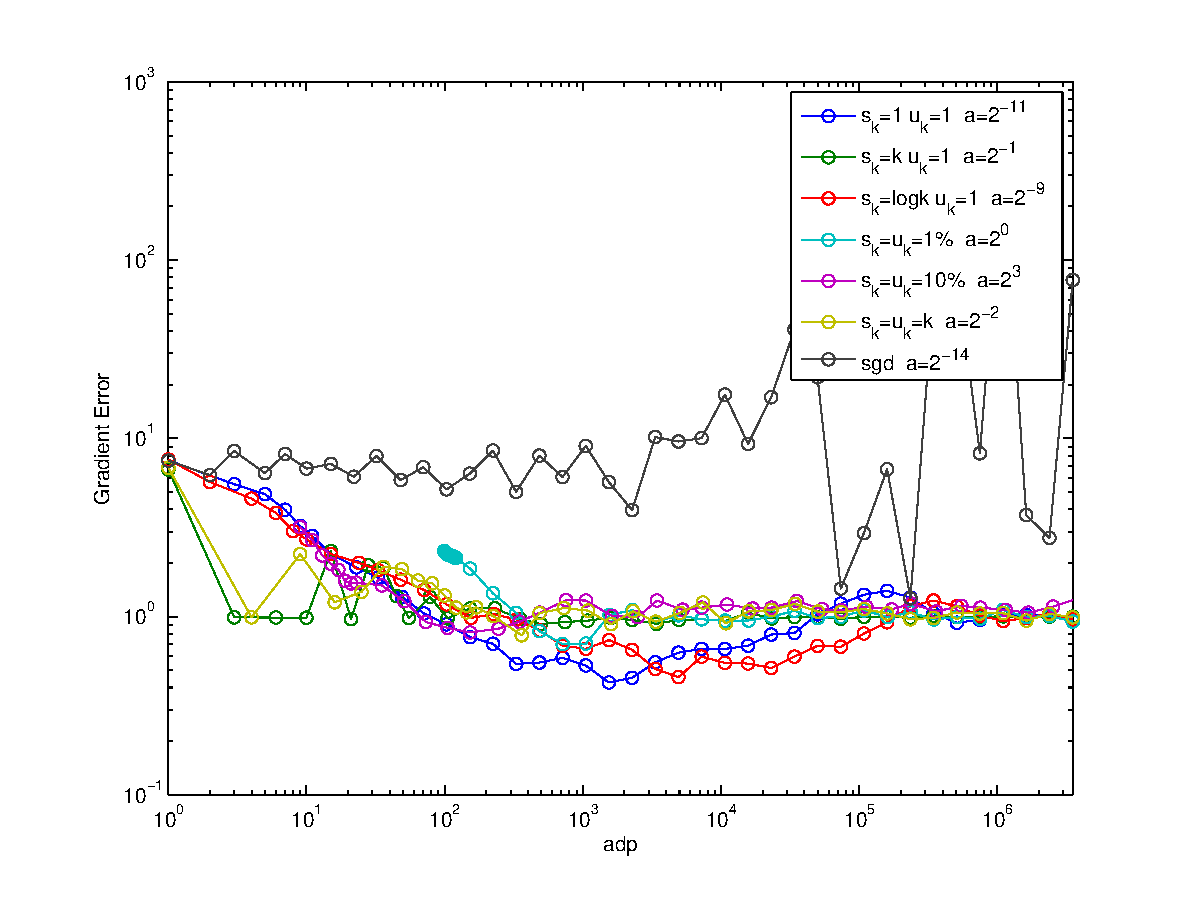
\includegraphics[width=4in]{Figures/16-3-3.eps}
	\end{subfigure}%
	\begin{subfigure}[b]{.5\linewidth}
		        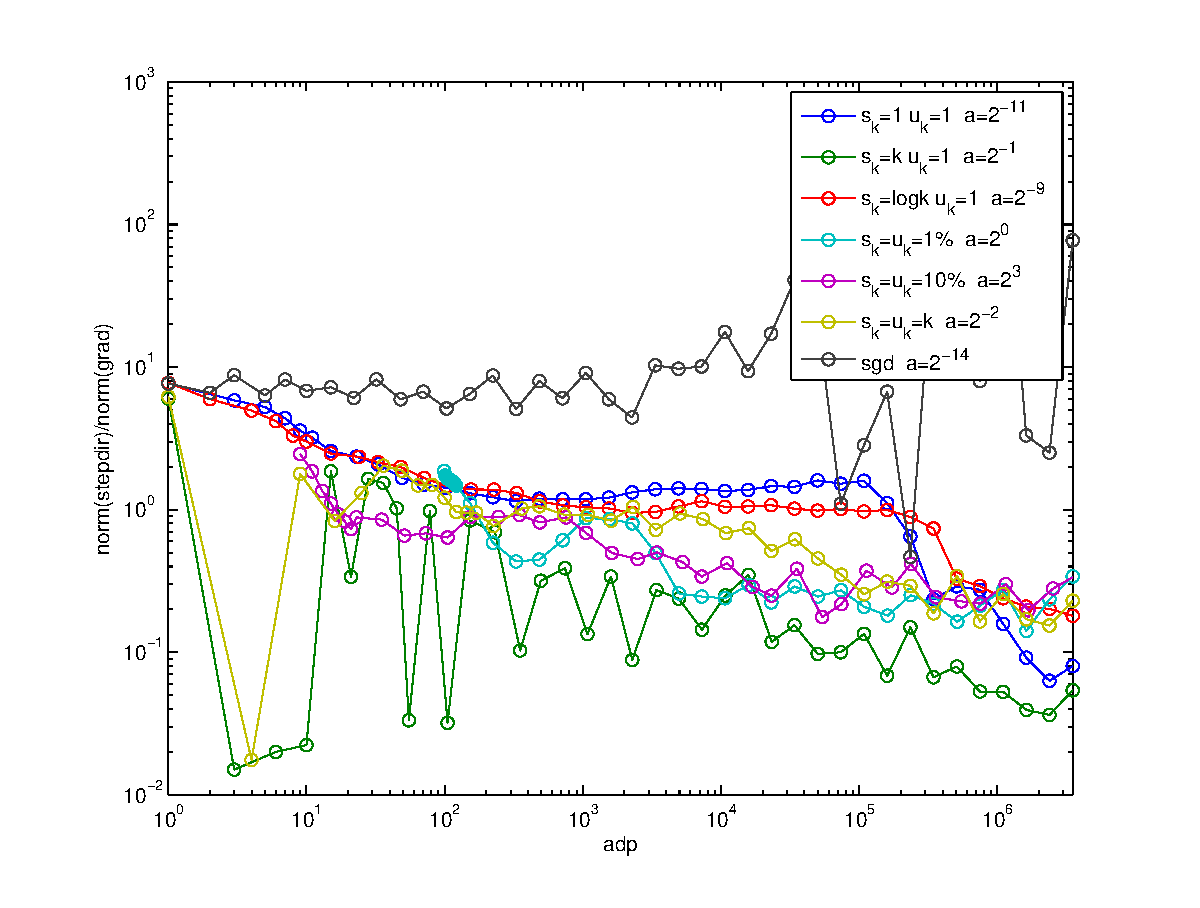
\includegraphics[width=4in]{Figures/16-3-4.eps}
	\end{subfigure}%
	\end{figure}
	
	SGD chooses the lowest stepsize we have seen, and the yellow method is still the same one.
	Blue and red methods become substantially shorter than the gradient - this effect can be correlated with setting $u_k=0$, but I'm not sure what the real cause and effect are here. \\
	The only loser here is the green method, the rest reach comparable excellent function values. 
	
	\newpage 
	
	\section{Call from Aug 7th}
	
	Drawback of SAG - want to extend to infinite summation of datapoints. That is one question. Generalization vs Training error, SAG might not be good for the former.
	
	Size of steplength depends on size of data set  - another drawback. 
	
	
	Motivation: algorithm that is not limited by the training set. 
	
	Figen's opinion on Johnson Zhang paper: Likes the idea of having strong information every once in a while. Makes steps go to zero without steplength go to zero. 
	
	Jorge: Johnson Zhang has a strong characteristic of computing a full batch. Analysis is on the cycles. 
	
	Write my function that I think is good to analyze, and motivate. 
	
	\subsection{Stefan Suggestion for Convergence Result}

	Consider the functions
	\begin{align*}
		F(\theta) & \defeq \mathbb{E}_{z}[ f(\theta;z)] \\
		F_I(\theta) & \defeq \frac{1}{\|I\|} \sum_{i \in I}  f(\theta, z_i).
	\end{align*}
	where $I$ is a set of sampled points $z_i$.
	
	
	There are many possible convergence (and convergence rate) results that might be provable for the ERG algorithm. Below are three possibilities:
	
	\begin{itemize}
		\item $F(\theta^k) - \min F(\theta) $ \\ these roughly correspond to the generalization error \\
		\item $F_{A}(\theta^k)- \min F_{A}(\theta) $ \\for some fixed set $A$. These are similar to SAG and SVRG results \\
		\item $F_{I_k}(\theta^k) - \min F_{I_k}(\theta)  $ \\ these are similar to the regret bound results in AdaGrad \\
	\end{itemize}
	
	I believe that we should stay clear of the second type of result, and instead focus on the first and the third options. The reason why the third option might be attractive is that it is closer to the actual functions we are working with, while still not having a requirement of looking at some pre-existing complete set of data points. 
	
	
	\newpage
	
	\section{Speech Problem} 
	
	Unregularized multi-class logistic regression with 143706 training points, 30315 variables. 
	
	\subsection{Exp}
	To reach the best function value
	\begin{figure}[H]
	\begin{subfigure}[b]{.5\linewidth}
		        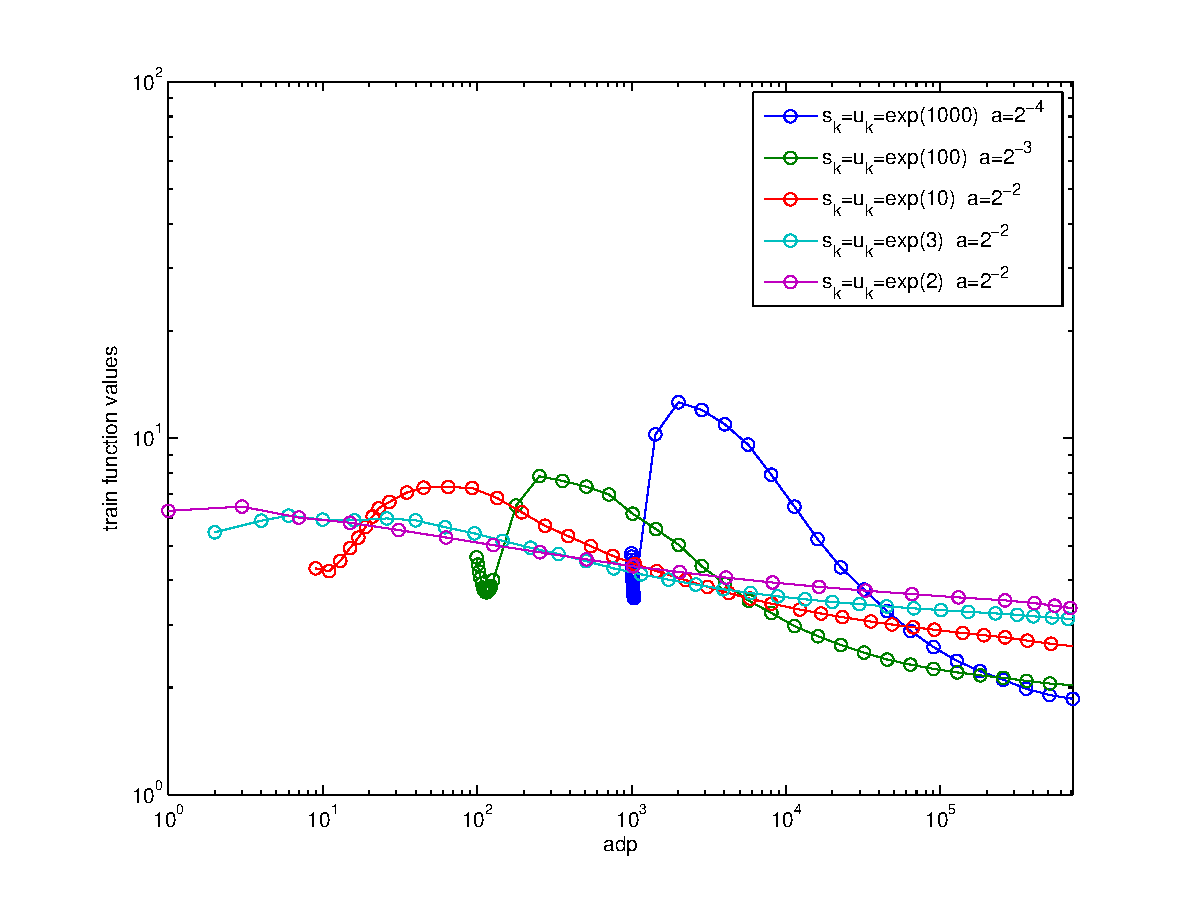
\includegraphics[width=4in]{Figures/18-1-1.eps}
	\end{subfigure}%
	\begin{subfigure}[b]{.5\linewidth}
		        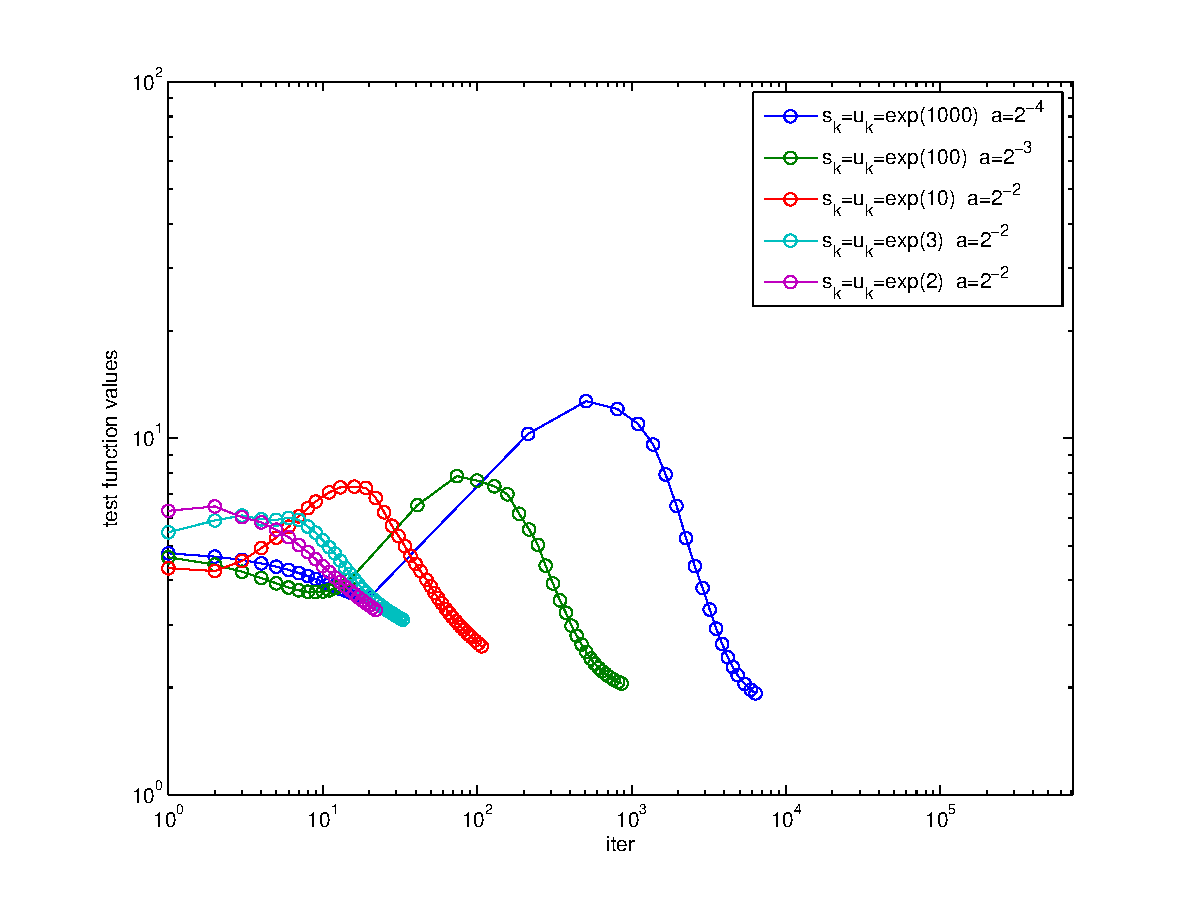
\includegraphics[width=4in]{Figures/18-1-2.eps}
	\end{subfigure}%

	\begin{subfigure}[b]{.5\linewidth}
		        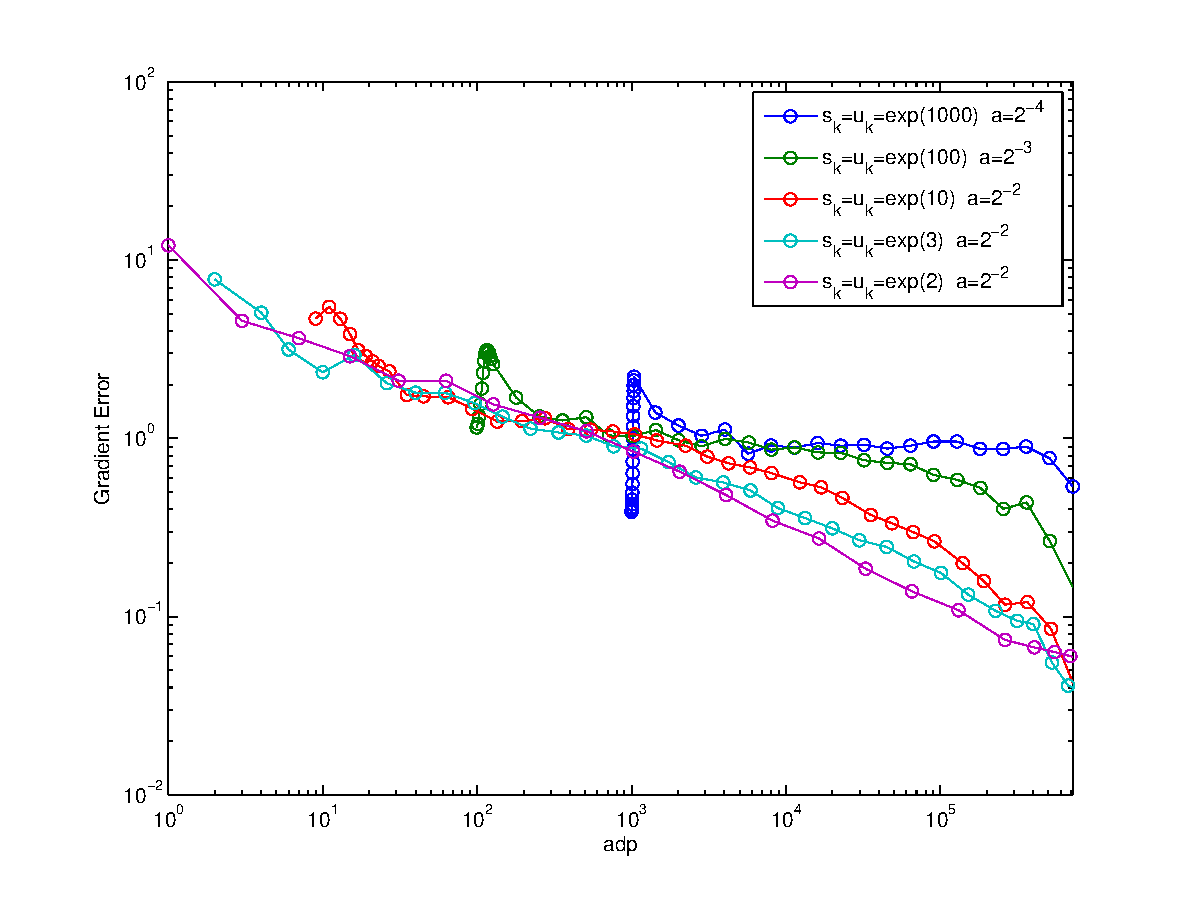
\includegraphics[width=4in]{Figures/18-1-3.eps}
	\end{subfigure}%
	\begin{subfigure}[b]{.5\linewidth}
		        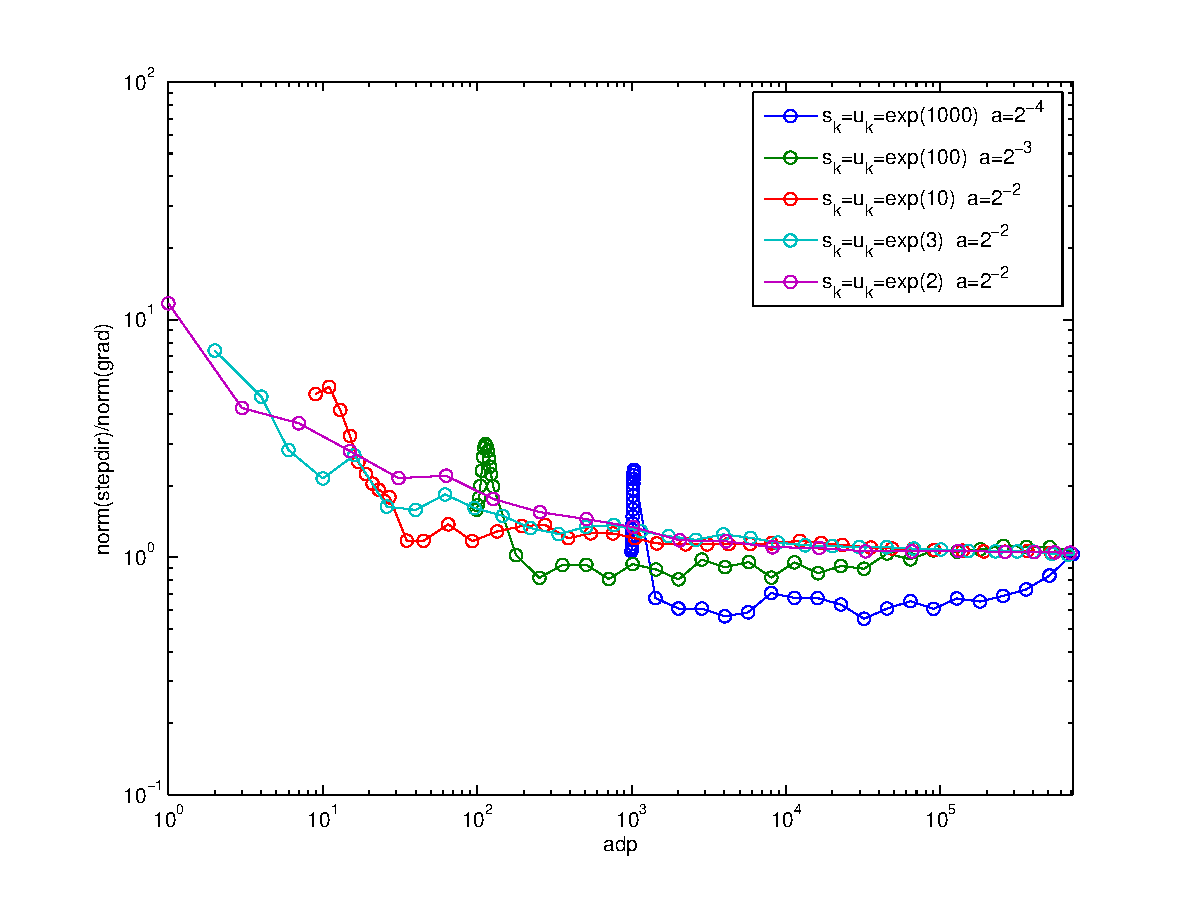
\includegraphics[width=4in]{Figures/18-1-4.eps}
	\end{subfigure}%
	\end{figure}
	
	\subsection{Different Strategies}
	To reach the best function value

	\begin{figure}[H]
	\begin{subfigure}[b]{.5\linewidth}
		        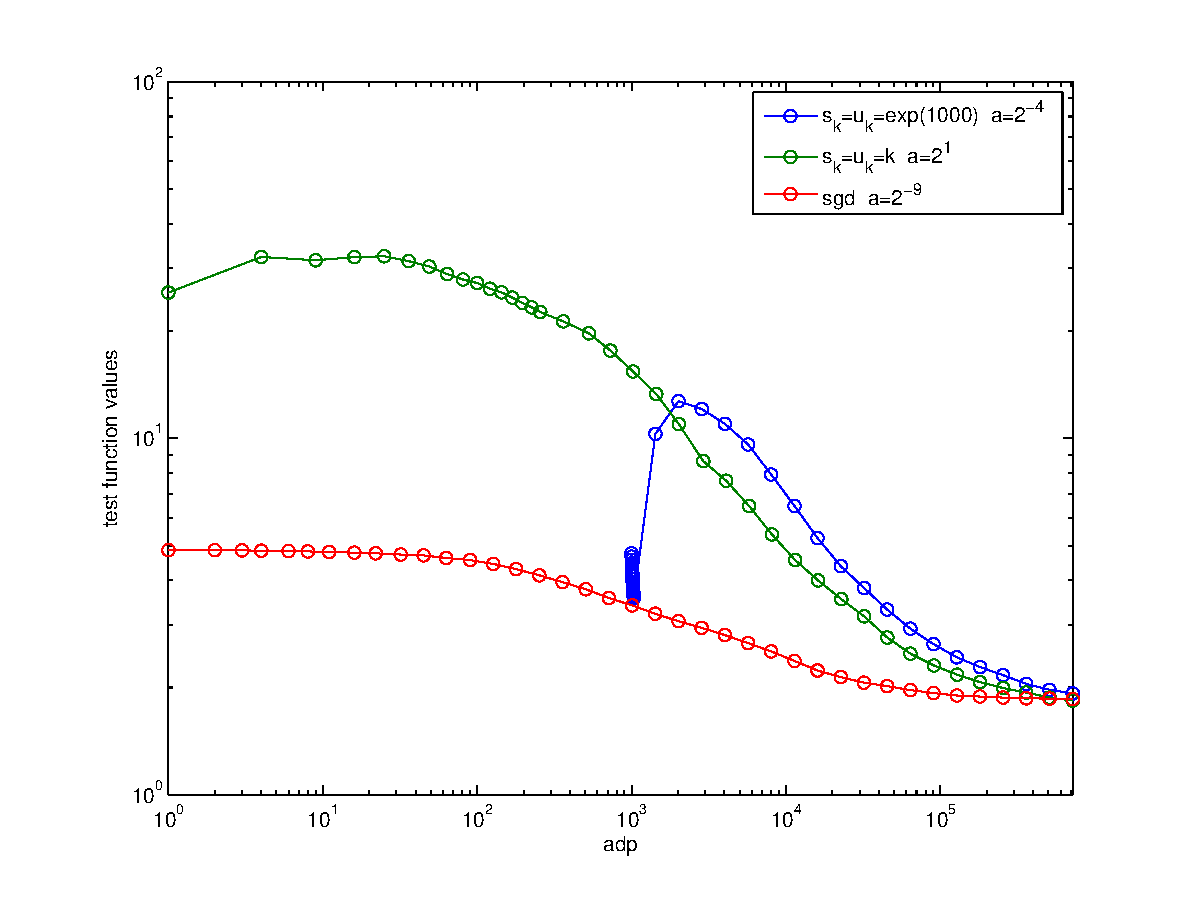
\includegraphics[width=4in]{Figures/18-2-1.eps}
	\end{subfigure}%
	\begin{subfigure}[b]{.5\linewidth}
		        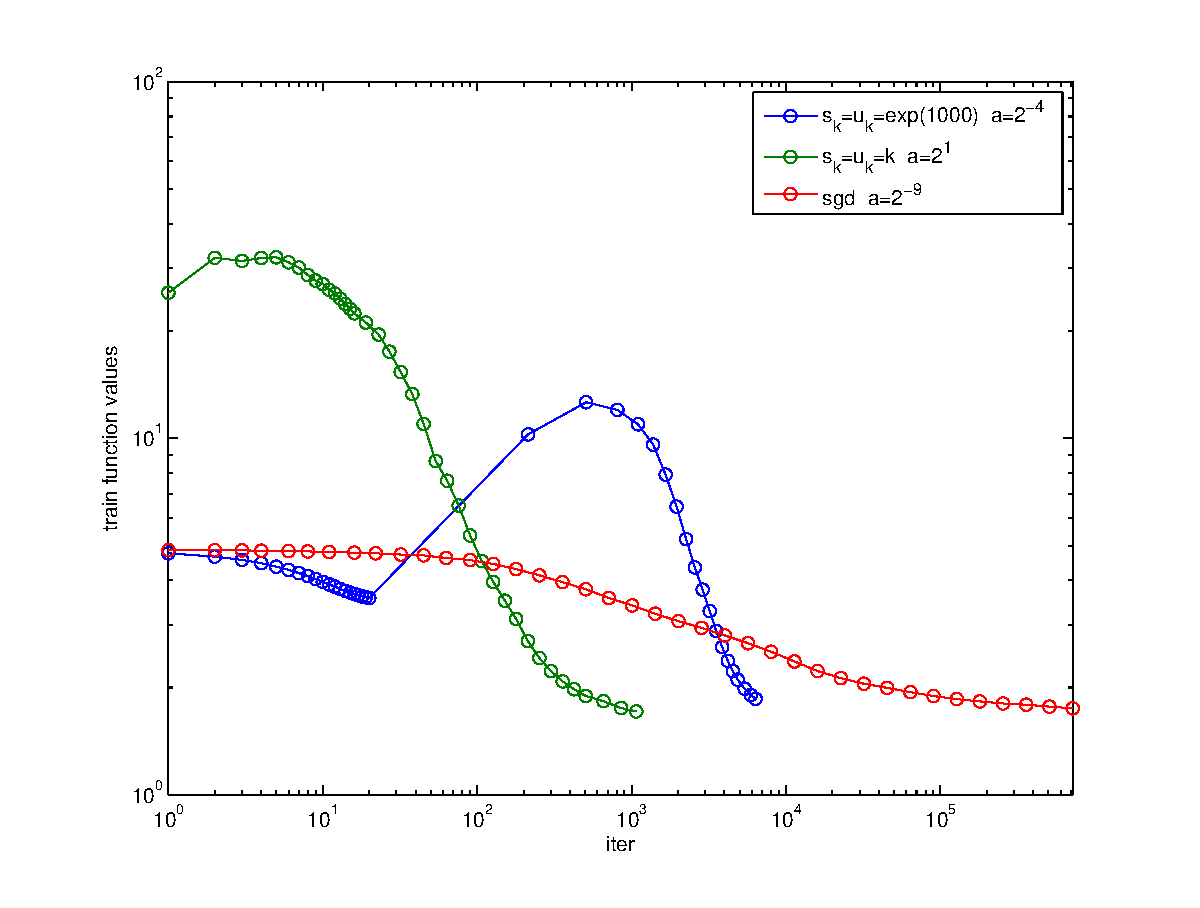
\includegraphics[width=4in]{Figures/18-2-2.eps}
	\end{subfigure}%

	\begin{subfigure}[b]{.5\linewidth}
		        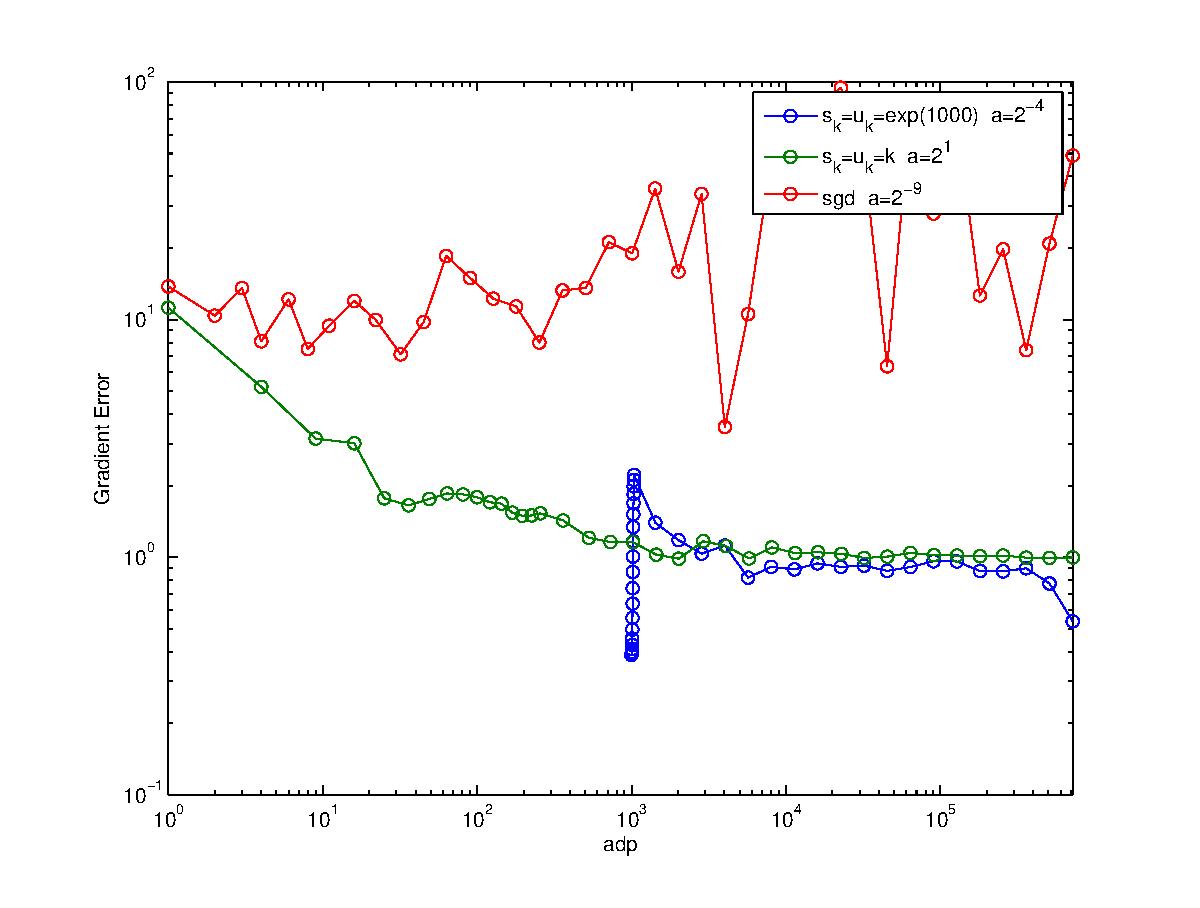
\includegraphics[width=4in]{Figures/18-2-3.eps}
	\end{subfigure}%
	\begin{subfigure}[b]{.5\linewidth}
		        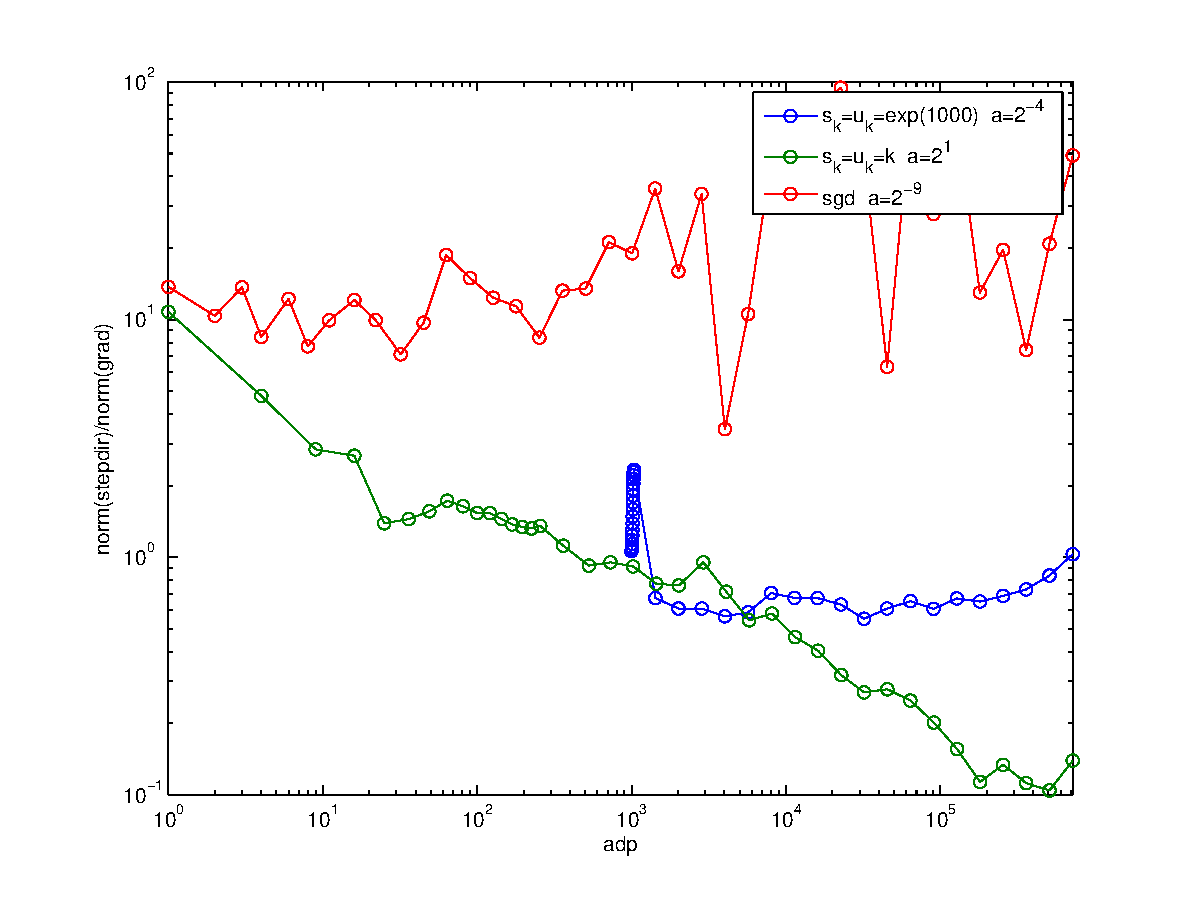
\includegraphics[width=4in]{Figures/18-2-4.eps}
	\end{subfigure}%
	\end{figure}
	
	\newpage
	
	\section{Alpha Problem}
	
	This is an L2 regularized binary logistic regression problem with 175000 training points, and 501 variables. Regularization parameter is 1e-2.
	
	
	\subsection{Exp}
	To reach the best function value
	\begin{figure}[H]
	\begin{subfigure}[b]{.5\linewidth}
		        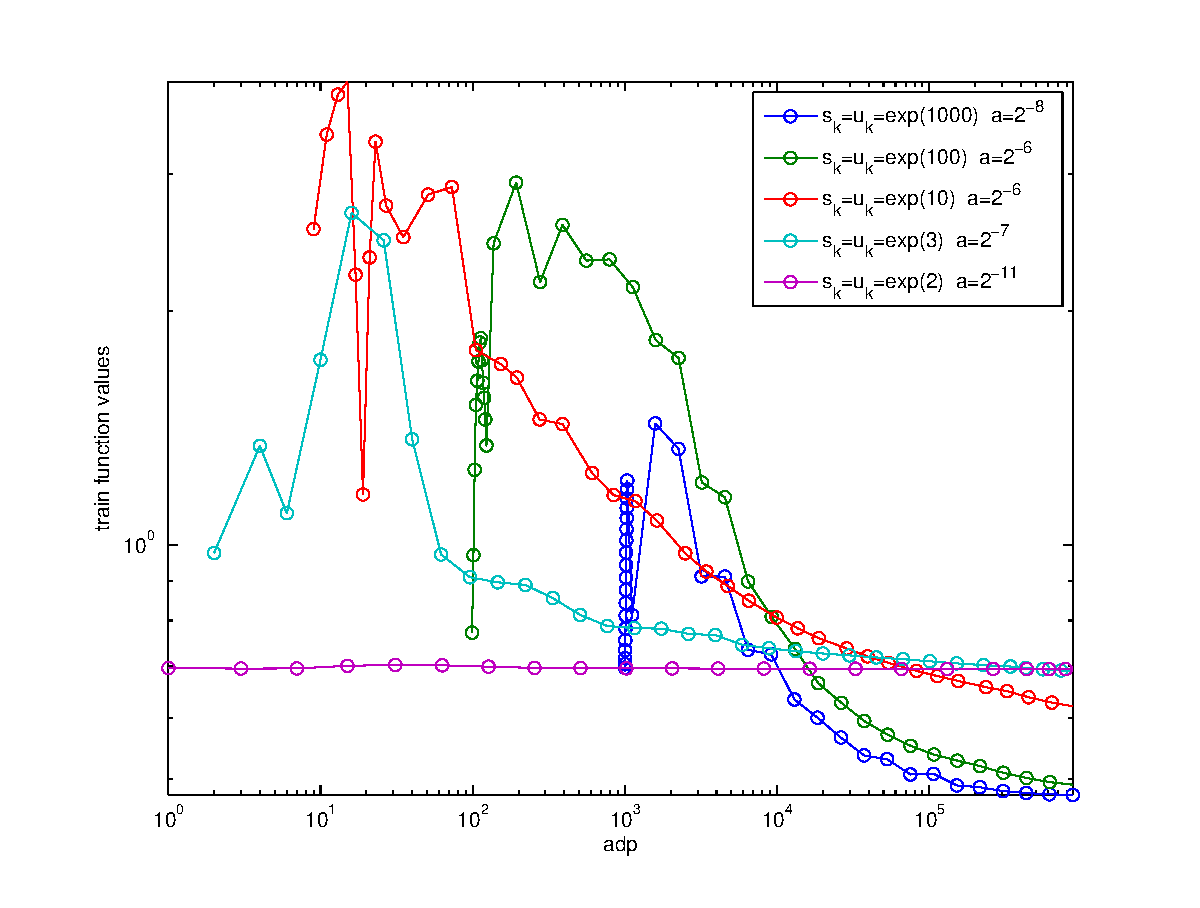
\includegraphics[width=4in]{Figures/19-1-1.eps}
	\end{subfigure}%
	\begin{subfigure}[b]{.5\linewidth}
		        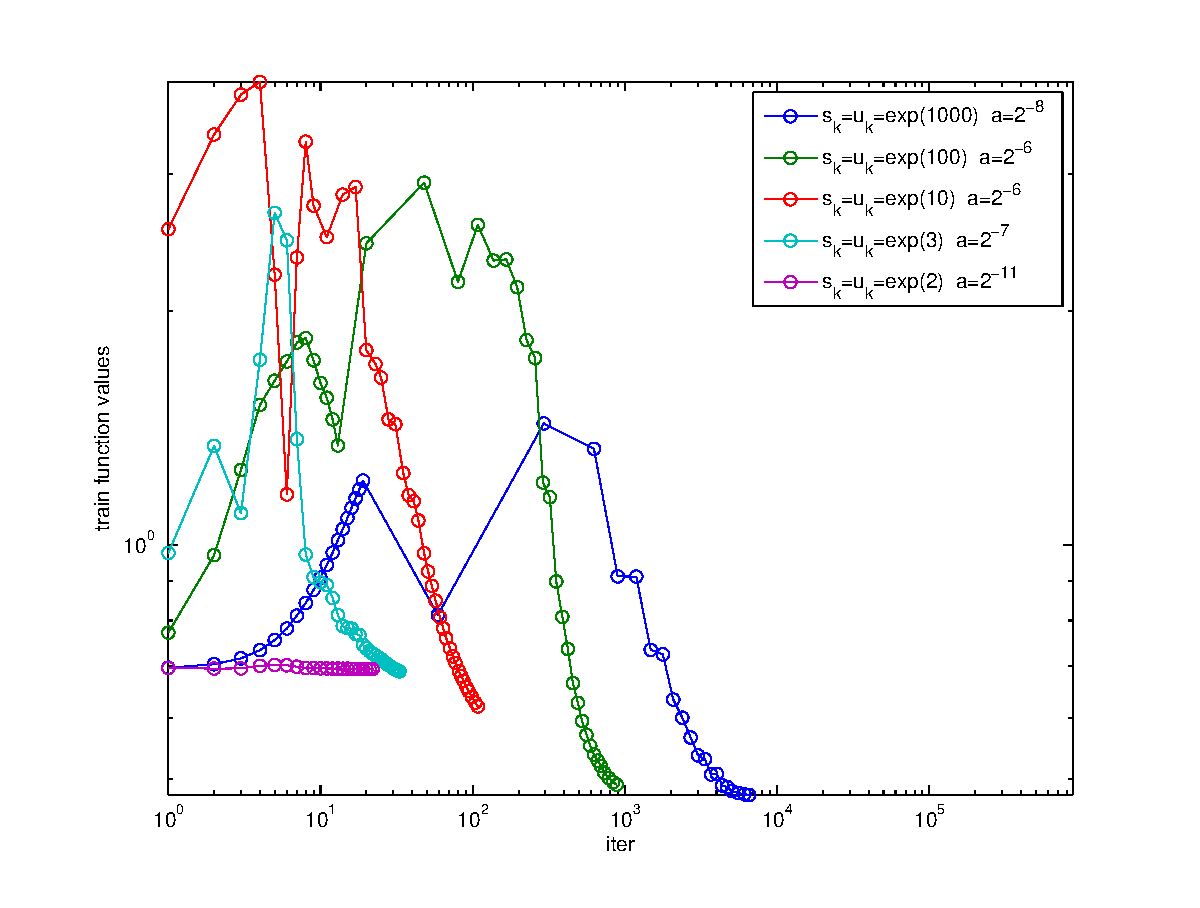
\includegraphics[width=4in]{Figures/19-1-2.eps}
	\end{subfigure}%

	\begin{subfigure}[b]{.5\linewidth}
		        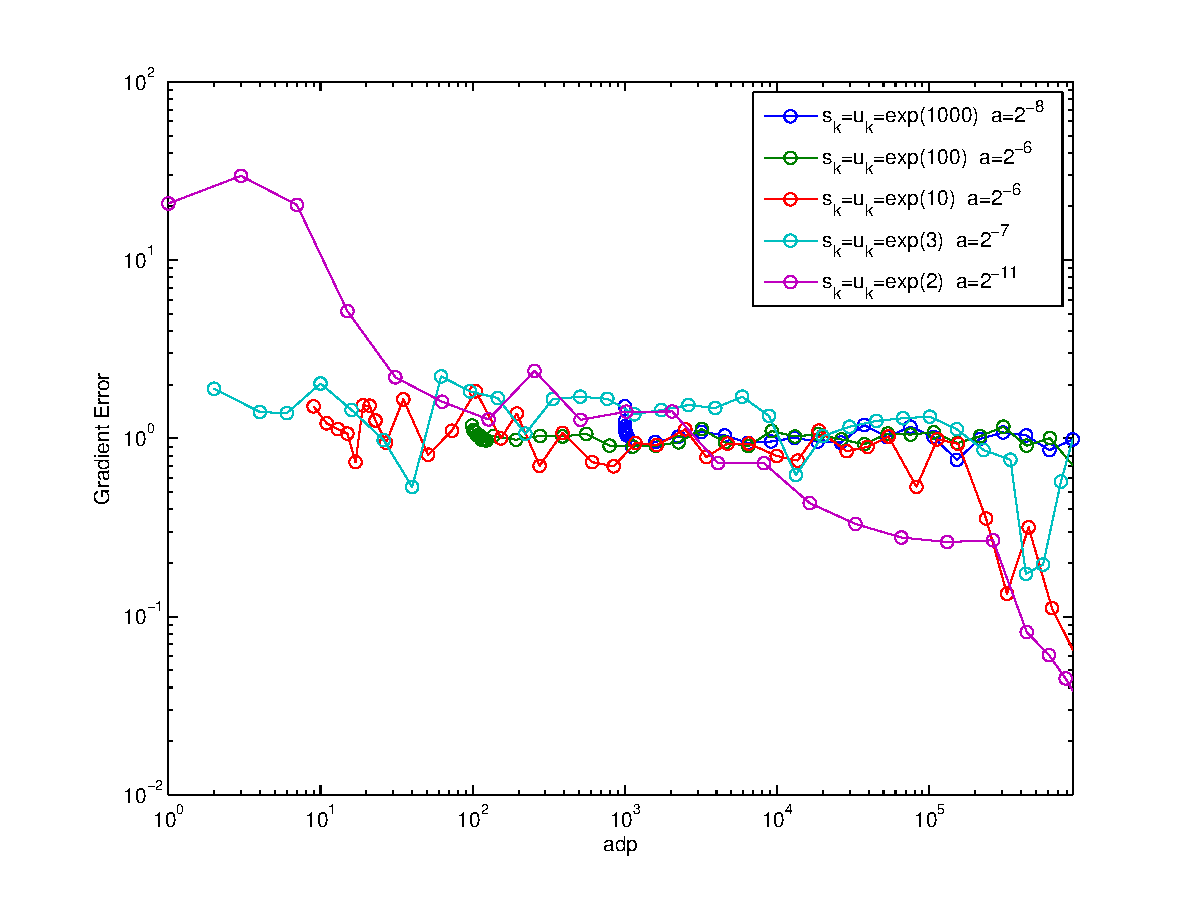
\includegraphics[width=4in]{Figures/19-1-3.eps}
	\end{subfigure}%
	\begin{subfigure}[b]{.5\linewidth}
		        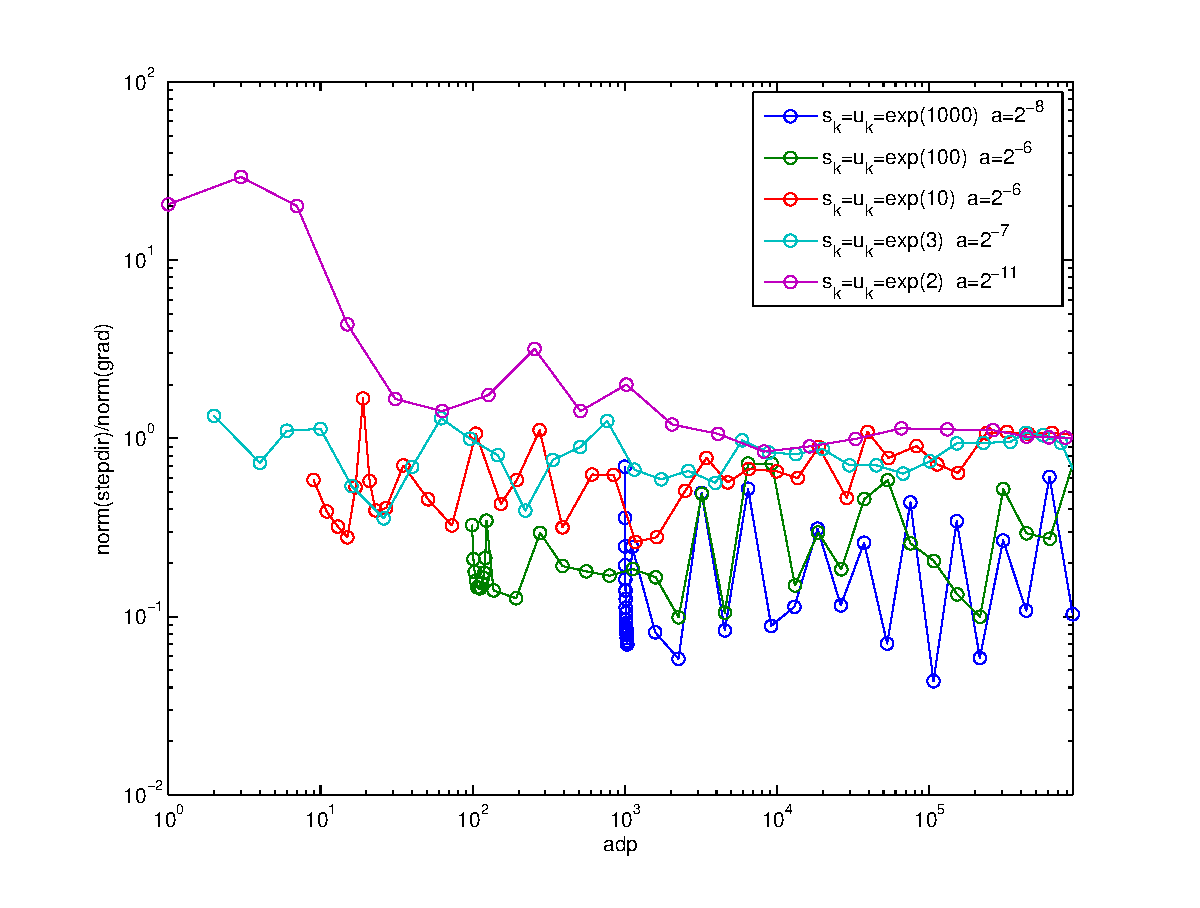
\includegraphics[width=4in]{Figures/19-1-4.eps}
	\end{subfigure}%
	\end{figure}
	
	\subsection{Different Strategies}
	To reach the best function value

	\begin{figure}[H]
	\begin{subfigure}[b]{.5\linewidth}
		        \includegraphics[width=4in]{Figures/19-2-1.eps}
	\end{subfigure}%
	\begin{subfigure}[b]{.5\linewidth}
		        \includegraphics[width=4in]{Figures/19-2-2.eps}
	\end{subfigure}%

	\begin{subfigure}[b]{.5\linewidth}
		        \includegraphics[width=4in]{Figures/19-2-3.eps}
	\end{subfigure}%
	\begin{subfigure}[b]{.5\linewidth}
		        \includegraphics[width=4in]{Figures/19-2-4.eps}
	\end{subfigure}%
	\end{figure}
	
\end{document}

%%%%%%%%%%%%%%%%%%%%%%%%%%%%%%%%%%%%%%%%%%%%%%%%%%%%%%%%%%%%%

